\fenicschapter{Cerebrospinal fluid flow}
              {Cerebrospinal fluid flow}
              {Cerebrospinal fluid flow}
              {Susanne St\o le-Hentschel, Svein Linge, Alf Emil L{\o}vgren and Kent-Andre Mardal}
              {hentschel}

This chapter concerns the flow of cerebrospinal fluid (CSF) in the
subarachnoid space that surrounds the spinal cord. Particular
attention is given to abnormal flow and pressure resulting from the
Chiari I malformation and its often associated condition
syringomyelia. The chapter builds on the software tools described in
Chapter~\ref{chap:kvs-1}, and we will compare the Chorin, IPCS and G2
methods. In this chapter, we will also describe how to create meshes
with Gmsh.

%------------------------------------------------------------------------------
\section{Medical background}

CSF is a clear water-like fluid that occupies the subarachnoid
space (SAS).  It surrounds the brain and the spinal cord, and also
fills the ventricular system within the brain. The SAS is bounded by
strong tissue layers, the dura mater as the outer boundary and the pia
mater as the inner boundary. A hole in the skull basis, foramen
magnum\index{foramen magnum}, connects the cranial and spinal parts of
the SAS. This hole is essential for CSF flow dynamics, since pulsating
blood vessels in the brain cause the brain to expand and contract, a
volume change that is made possible only by a simultaneous pulsating
flow of CSF through the foramen magnum. Hence, the pulse that travels
through the blood vessel network is transformed to a pulse in the CSF
system, a pulse that is dampened on its way along the spinal
canal. The CSF also plays an important role in cushioning the brain
and the spinal cord.
\index{spinal canal}
\index{cerebrospinal fluid}
\index{CSF}
\index{subarachnoid space}
\index{SAS}

\begin{figure}
\bwfig
  \centering
  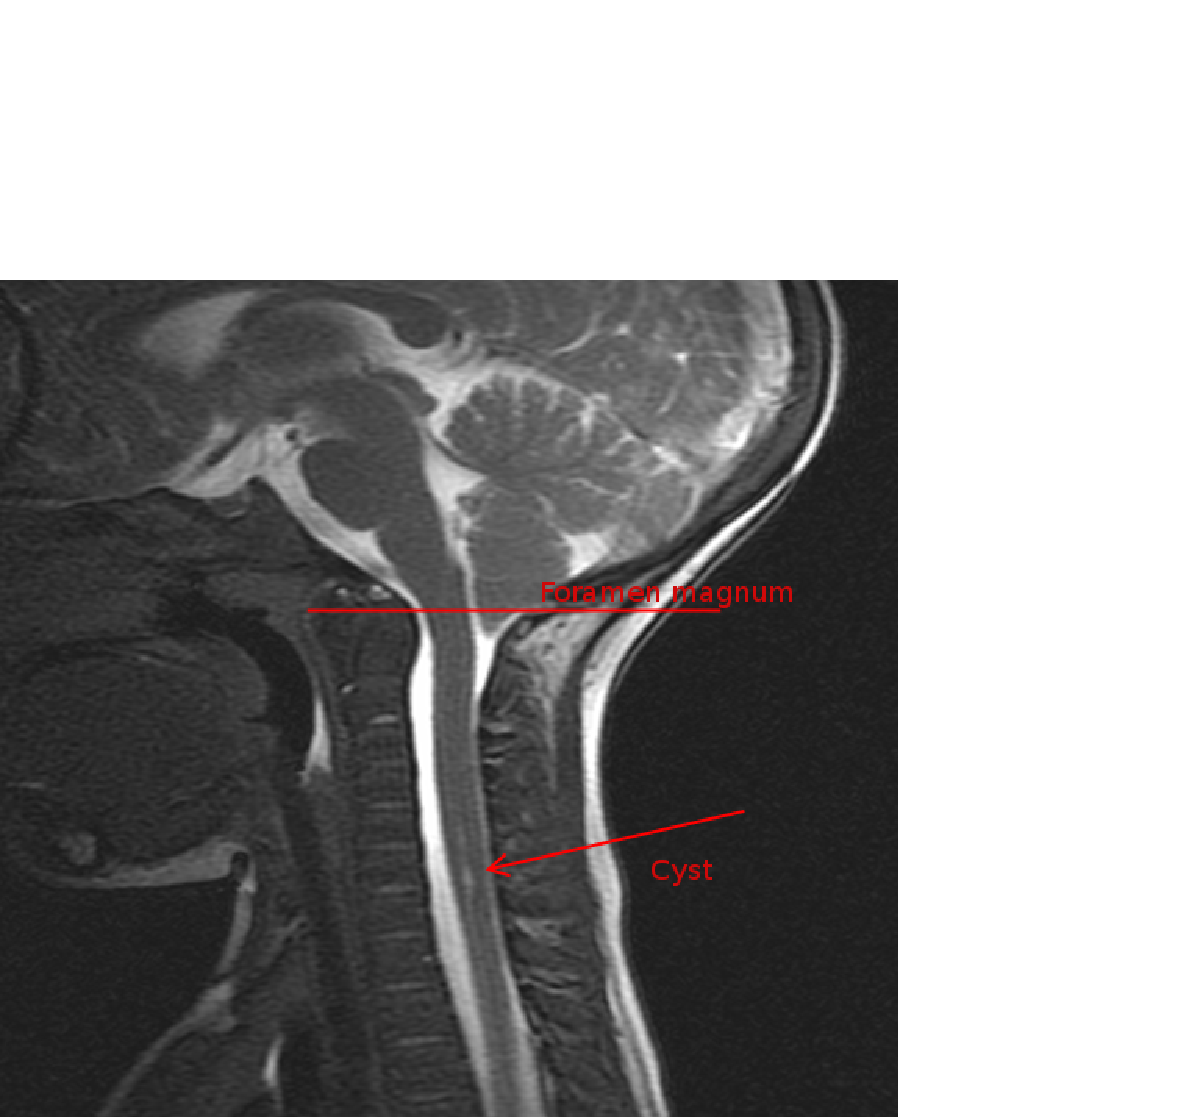
\includegraphics[width=\largefig]{chapters/hentschel/pdf/ChiariImage2.pdf}
  \caption{The picture shows an MR image of a patient with a Chiari I
    malformation. Chiari I patients are characterized by a very narrow
    passage at the foramen magnum; that is, the subarachnoid space, shown
    as white on the image, is small compared to normals. Chiari patients
    often develop cysts within the spinal cord, visible as white spots in
    the dark grey cord. Notice the relatively large distance between the
    narrow foramen magnum and the cyst.}
  \label{fig:anatomy}
\end{figure}

The left picture in Figure~\ref{fig:anatomy} shows the CSF and the
main structures in the brain of a healthy individual. In about 0.6\%
of the population the lower part of the cerebellum occupies parts of
the CSF space in the upper spinal SAS and obstructs the CSF flow. This
so-called Chiari I malformation \index{Chiari I malformation} (or
Arnold-Chiari malformation) is shown in the right picture in
Figure~\ref{fig:anatomy}. A variety of symptoms are related to this
malformation, including headache, abnormal eye-movement, motor or
sensor-dysfunctions, etc. If the malformation is not treated
surgically, the condition may become more severe and cause serious
neurological deterioration, and may even lead to death.

Many people with the Chiari I malformation develop fluid filled
cavities, often called syrinxes or cysts, within the spinal cord,
\index{spinal cord} a condition called syringomyelia. The exact
relation between the Chiari I malformation and syringomyelia is not
known. It is believed that flow and pressure disturbances caused
by abnormal obstructions initiate the development of syringomyelia
\citep{OldfieldMuraszkoShawkerEtAl1994}. Several authors have
analyzed the relations between abnormal flow and syringomyelia
development based on measurements in patients and healthy volunteers
\citep{HeissPatronasDeVroomEtAl1999,PinnaAlessandriniAlfieriEtAl2000,HofmannWarmuth-MetzBendszusEtAl2000,HaughtonKorosecMedowEtAl2003}.
These studies also compare flow dynamics before and after decompressive
surgery. The latter is an operation, where the SAS lumen around the
obstructed area is increased by removing parts of the surrounding
tissue and bone~\citep{MilhoratBolognese2003}. Control images
taken some weeks or months after the intervention often show
a reduction of the size of the cyst in the spinal canal and
patients usually report improvement of their condition. In
some cases, the syrinx disappeared completely after some months
\citep{OldfieldMuraszkoShawkerEtAl1994,PinnaAlessandriniAlfieriEtAl2000,HeissPatronasDeVroomEtAl1999}.

Several studies \citep{Quigley2004,HaughtonKorosecMedowEtAl2003}
report that the measured CSF flow at foramen magnum is abnormal
in the sense that the flow contains high speed jets and also
synchronous bidirectional flow.  Computational fluid dynamics
(CFD) simulations have related the abnormal flow to abnormal pressure
\citep{RoldanHaughtonWiebenEtAl2009,HentschelMardalLovgren2010,LingeHaughtonLovgren2010,LingeHaughtonLovgren2011}.
Many theories have been proposed to describe the relation between the
Chiari I malformation and syringomyelia. However, it is hard to explain
the relatively large distance between the Chiari I malformation and
the cyst.

It is the purpose of this chapter to show how relevant CFD solvers in
\fenics may be used to investigate unresolved issues in CSF flow dynamics.
Specifically, we investigate different boundary conditions, different
geometries, and also how far velocity and pressure disturbances travel
under realistic conditions. We also compare the different numerical
schemes Chorin, IPCS and G2 described in Chapter~\ref{chap:kvs-1}.

\section{Mathematical description}

We model the CSF flow in the upper spinal canal as a Newtonian fluid
\index{Newtonian fluid} with viscosity and density similar to water
at body temperature. The upper spinal canal is represented as a tube
with an inner elliptic or circular cylinder removed.  In the presented
experiments, we focus on the dynamics around the spinal cord. The
tissue surrounding the fluid is modeled as impermeable and rigid
throughout the cardiac cycle.

To simulate CSF flow, we apply the
Navier--Stokes  equations for an incompressible
Newtonian fluid,
\begin{equation}
  \begin{split}
    \rho \left(\frac{\partial v}{\partial t} + v \cdot \nabla v \right)
          &= -\nabla p + \mu \Delta v + g,
    \\
    \nabla \cdot v &= 0,
  \end{split}
\end{equation}
with the variables as indicated in Table~\ref{tab:entities}, and $g$,
the body force; that is, gravity.  We can eliminate gravity from the
equation by assuming that the body force is balanced by the hydrostatic
pressure.  As a result, pressure describes only the dynamic pressure. To
calculate the correct physical pressure, static pressure resulting from
body forces has to be added. This simplification is not true, however,
during sudden movements such as standing up.

\begin{table}
  \centering
  \begin{tabular}{ccccc}
    \toprule
    Symbol & Meaning & Unit & Value Used & Reference \\
    \midrule
    $\mathbf{v}$	& velocity variable & $\mathrm{\frac{cm}{s}}$ & --- & $-1.3\pm 0.6 \ldots 2.4 \pm 1.4$  \\
    $p$		& pressure	variable & $\mathrm{\frac{dyne}{cm^2}}$ & --- & \ldots\\
    $\rho$	& density & $\mathrm{\frac{g}{cm^3}}$ & --- &0.993 \\ %\textcelsius
    $\mu$	& dynamic viscosity	&  $\mathrm{\frac{g s}{cm}}$ & --- & 0.0007\\
    $\nu$	& kinematic viscosity & $\mathrm{ \frac{cm^2}{s}}$ & $0.7 10^{-2}$ & $0.7 10^{-2}$ \\ 	\midrule %$(\nu = \frac{\mu}{\rho})$
    $SV$	& stroke volume 	& $\mathrm{\frac{ml}{s}}$& $0.27$  & $0.27$ \\
    $HR$	& heart rate & $\mathrm{\frac{beats}{s}}$	& 1.17 & 1.17\\
    $A0$	& tube boundary	& $\mathrm{cm^2}$ & $32$  & ---\\
    $A1$,$A2$	& area of inlet/outlet & $\mathrm{cm^2}$ &$0.93$ & 0.8 \ldots 1.1   \\
    \midrule
    $Re$    & Reynolds Number & -- & -- & ~70--200 \\
    $We$    & Womersley Number & -- & -- & ~14--17 \\
    \bottomrule
  \end{tabular}
  \caption{Characteristic values and parameters for CSF flow
    modeling.  The velocities are maximum absolute anterior CSF flow
    velocities taken from controls and Chiari I malformation patients
    \citep{HofmannWarmuth-MetzBendszusEtAl2000}.  By stroke volume
    we mean the volume that moves up and down through cross section
    in the SAS during one cardiac cycle and the value is taken from
    \citep{GuptaSoellingerBoesigerEtAl2009}.  Cross section areas 20--40 cm
    from the foramen magnum are taken from \citep{LothYardimciAlperin2001}.}
  \label{tab:entities}
\end{table}
% reference: http://www.thermexcel.com/english/tables/eau_atm.htm

\section{Numerical experiments}

\subsection{Implementation}

We refer to Chapter~\ref{chap:kvs-1} for a complete description of the
solvers and schemes implemented. In this chapter we concentrate on the use
of these solvers in a few examples. Notice, however, that we use first
order velocity elements, since the results with first order elements
was virtually identical to the results with second order elements in
this case.  The code can be found in \emp{csf\_flow.py}.

\paragraph{Boundary conditions.}
The mesh boundaries at the inlet cross section, the outlet cross
section, and the SAS boundaries are defined by the respective
classes \emp{Top}, \emp{Bottom}, and \emp{Contour}. They are
implemented as subclasses of \emp{SubDomain}, similarly to the given
example of \emp{Top}.
\begin{python}
class Top(SubDomain):
    def __init__(self, z_index, z_max, z_min):
        SubDomain.__init__(self)
        self.z_index = z_index
        self.z_max = z_max
        self.z_min = z_min

    def inside(self, x, on_boundary):
        return bool(on_boundary and x[self.z_index] == self.z_max)
\end{python}
To define the domain correctly, we override the base class
function \emp{inside}. It returns a boolean evaluating if the inserted
point \emp{x} is part of the subdomain. The boolean \emp{on\_boundary}
is very useful to easily partition the whole mesh boundary to
subdomains.

It would be physically more correct to require that the no slip
condition also is valid on the outermost/innermost nodes of the inflow
and outflow sections as implemented below:
\begin{python}
def on_ellipse(x, a, b, x_index, y_index, x_move=0, y_move=0):
    x1 = x[x_index] - x_move
    x2 = x[y_index] - y_move
    return bool( abs((x1/a)**2 + (x2/b)**2 - 1.0 ) < 10**-6 )
\end{python}
The vectors describing the ellipses of the cord and the dura in a
cross section with the corresponding axes are required. The global
function \emp{on\_ellipse} checks if \emp{x} is on the ellipse defined
by the x-vector \emp{a} and the y-vector \emp{b}. The
variables \emp{x\_move} and \emp{y\_move} allow the definition of an
eccentric ellipse.

Defining the inflow area at the top, with mantle nodes excluded, is
done as shown in the following code. The outflow area at the bottom is
defined analogously.

\begin{python}
class Top(SubDomain): # bc for top
    def __init__(self, a2_o, a2_i, b2_o, b2_i, x_index, y_index, z_index, z_max, \
                x2_o_move=0, y2_o_move=0, x2_i_move=0, y2_i_move=0):
        SubDomain.__init__(self)
        self.x_index = x_index
        self.y_index = y_index
        self.a2_o = a2_o
        self.a2_i = a2_i
        self.b2_o = b2_o
        self.b2_i = b2_i
        self.z_index = z_index
        self.z_max = z_max
        self.x2_o_move = x2_o_move
        self.x2_i_move = x2_i_move
        self.y2_o_move = y2_o_move
        self.y2_i_move = y2_i_move

    def inside(self, x, on_boundary):
        return on_boundary and abs(x[self.z_index] - self.z_max) < 10**-6 \
               and not on_ellipse(x, self.a2_o, self.b2_o, self.x_index, \
                              self.y_index, self.x2_o_move, self.y2_o_move) \
               and not on_ellipse(x, self.a2_i, self.b2_i, self.x_index, \
                              self.y_index, self.x2_i_move, self.y2_i_move))
\end{python}

The underscores \emp{o} and \emp{i} represent the outer and inner
ellipse, respectively. The numbering with \emp{2} distinguishes the
subdomain at the top from that at the bottom, which may be defined
differently. The details of how different problems can easily be
defined in separate classes can be found in
\emp{src/mesh\_definitions/}. %FIXME

According to \citet{GuptaSoellingerBoesigerEtAl2009}, a volume of 0.27
ml is transported back and forth through the spinal SAS cross sections
during each cardiac cycle. For the average human, we assume a heart
rate of 70 beats per minute. Furthermore, we define the cross
sectional area to be $0.93\,\mathrm{cm^2}$, which matches a segment
from 20 to 40 cm down from the foramen
magnum~\citep{LothYardimciAlperin2001}. In this region of the spinal
canal, the cross sectional area varies little. In addition, the dura
and the cord shape resembles a simple tube more than in other regions.
According to \citet{OldfieldMuraszkoShawkerEtAl1994}, syrinxes start
at around 5 cm below the foramen magnum and extend up to 28 cm below
the foramen magnum.

Moreover, we define a velocity pulse on the inflow and outflow
boundaries, and since we are modeling incompressible flow between
rigid impermeable boundaries, we must have equal inflow and outflow
volumes at all times. The pulse values in these boundary cross
sections were set equal in every grid point, and scaled to match the
volume transport of 0.27 ml.

\begin{figure}
\bwfig
  \centering
  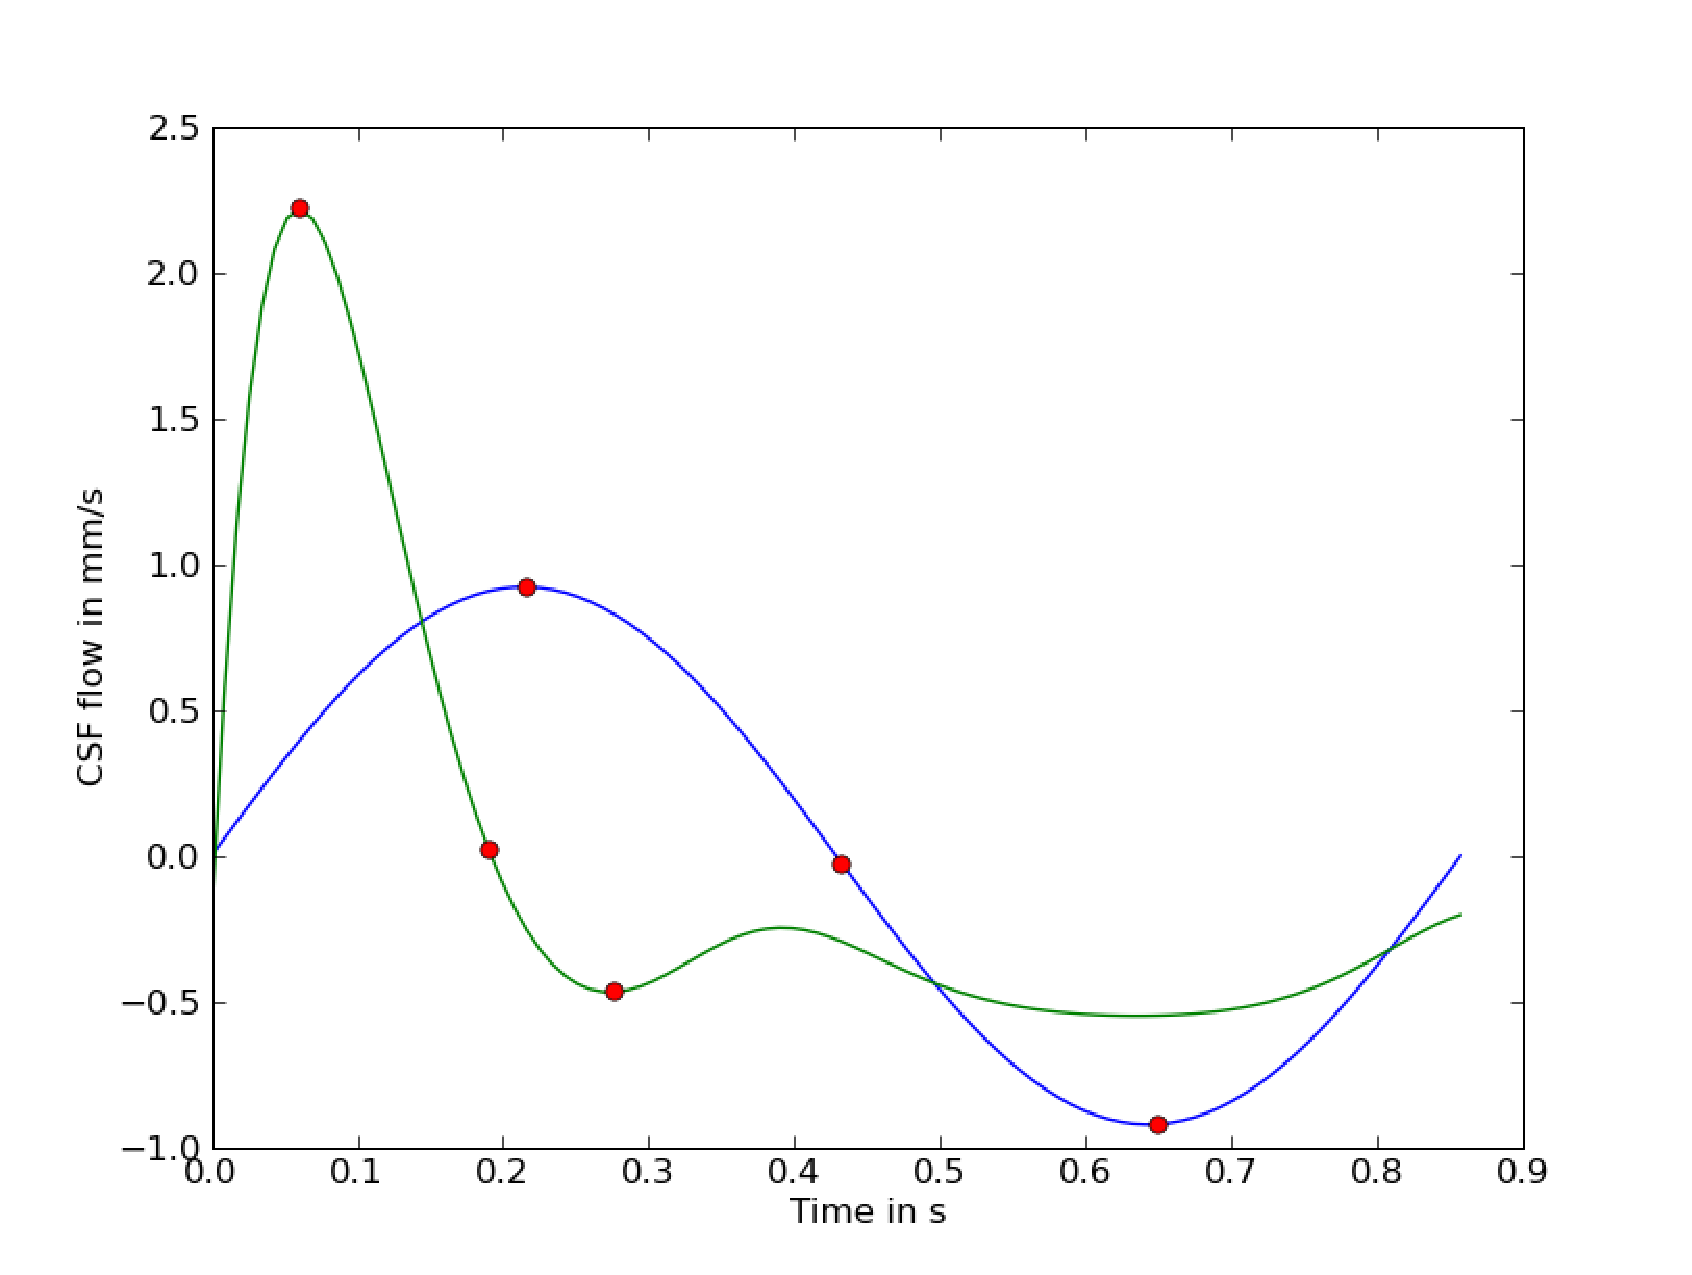
\includegraphics[width=\largefig]{chapters/hentschel/pdf/sin_pulse.pdf}
  \caption{Two different CSF flow pulses. The blue line is a sine pulse,
    whereas the green is derived from the pressure pulse in a heart
    chamber.}
  \label{fig:sin_pulse}
\end{figure}

A function describing the varying blood pressure in a heart chamber is
given in \citet{SmithChase2ShawEtAl2006}.  With some adjustment and
additional parameters, the function was adapted to approximate the CSF
flow pulse, see Figure~\ref{fig:sin_pulse}.  The systole of the pulse
function is characterized by a high amplitude with a short duration
while the negative counter movement has a reduced amplitude and lasts
considerably longer.  The global function for defining the pulse is:
\begin{python}
def get_pulse_input_function(V, z_index, factor, A, HR_inv, HR, b, f1):
    C0 = 3.4 * pi
    rad = C0 /HR_inv
    v_z = "factor*(-A*(exp(-fmod(t, T)*rad)*Ees*(sin(-f1*fmod(t, T)*rad) - vd)
     - (1-exp(-factor*fmod(t, T)*rad))*p0*(exp(sin(-fmod(t, T)*rad) - vd) -1)) - b)"
    vel = ["0.0", "0.0", "0.0"]
    vel[z_index] = v_z
   defaults = {"factor":factor, "A":A, "p0":1, "vd":0.03, "Ees":50,
               "T": HR_inv, "HR":HR, "rad":rad, "b":b, "f1":f1}
    pulse = Expression(vel, defaults)
    return pulse
\end{python}
The following parameters have been used with this function.
\begin{python}
A = 2.9/16
factor = self.flow_per_unit_area/0.324
v_max = 2.5 * self.factor
b = 0.465
f1 = 0.8
\end{python}

\paragraph{Initialization of the problem.}
The \emp{Problem} class in \emp{csf\_flow}, derived from \emp{ProblemBase}
in \emp{nsbench} described in Chapter~\ref{chap:kvs-1}, defines the
mesh with its boundaries and provides the necessary information for
the Navier--Stokes solvers. The mesh is ordered for all entities and
initiated to compute its faces.

The values \emp{z\_min} and \emp{z\_max} mark the inflow and outflow
coordinates along the tube's length axis. As mentioned above, the axis
along the tube is indicated by \emp{z\_index}. If one of the coordinates,
or the z-index, is not known, it may help to call the mesh in viper
\emp{unix>viper meshname.xml}. Typing \emp{o} prints the length in
x, y and z direction in the terminal window. Defining \emp{z\_min},
\emp{z\_max} and \emp{z\_index} correctly is important for the classes
that define the boundary domains of the mesh \emp{Top}, \emp{Bottom}
and \emp{Contour}. As we have seen before, \emp{z\_index} is necessary
to set the correct component to the nonzero boundary velocity.

Exterior forces on the Navier--Stokes flow are defined in the object
variable \emp{f}. Since gravity is neglected in the current problem
formulation, the force function \emp{f} is defined by a constant function
\emp{Constant} with value zero on the complete mesh.

After initializing the subdomains, \emp{Top}, \emp{Bottom} and
\emp{Contour}, they are marked with reference numbers attributed to the
collection of all subdomains \emp{sub\_domains}.

To see the most important effects, the simulation was run slightly
longer than one full period. A longer simulation time was not found
necessary, since undesirable effects of the physiologically incorrect
starting value (zero velocity) was dampened sufficiently already very
early in the first period. Besides maximum and minimum velocities, the
simulation includes the transition from diastole to systole, and vice
versa.  With the given physiological time scales of the problem, the
chosen time step length (0.001 s) represents a high temporal
resolution.
\begin{python}
def __init__(self, options):
    ProblemBase.__init__(self, options)
    filename = "../../data/meshes/chiari/csf_extrude_2d_bd1.xml.gz"
    self.mesh = Mesh(filename)
    self.mesh.order()
    self.mesh.init(2)

    self.z_max = 5.0	# in cm
    self.z_min = 0.0	# in cm
    self.z_index = 2
    self.D = 0.5 		# characteristic diameter in cm

    self.contour = Contour(self.z_index, self.z_max, self.z_min)
    self.bottom = Bottom(self.z_index, self.z_max, self.z_min)
    self.top = Top(self.z_index, self.z_max, self.z_min)

    # Load subdomain markers
    self.sub_domains = FacetFunction("uint", self.mesh)

    # Mark all facets as subdomain 3
    for i in range(self.sub_domains.size()):

        self.sub_domains.set(i, 3)
        self.contour.mark(self.sub_domains, 0)
        self.top.mark(self.sub_domains, 1)
        self.bottom.mark(self.sub_domains, 2)

        # Set viscosity
        self.nu = 0.7 * 10**-2 # cm^2/s

        # Create right-hand side function
        self.f = Constant((0.0, 0.0, 0.0))
        n = FacetNormal(self.mesh)

        # Set end-time
        self.T = 1.2 * 1.0/self.HR
        self.dt = 0.001
\end{python}

Increasing the time step length usually speeds up the calculation of
the solution. As long as the CFL number with the maximum velocity
$v_{max}$, time step length $dt$ and minimal edge length $h_{min}$ is
smaller than one $(CFL = \frac{v_{max} dt}{h_{min}} < 1)$, the solvers
should converge. Too small time steps, however, can lead to an
increasing number of iterations for the solver on each time step.  As
a characterization of the fluid flow, the Reynolds number $(Re =
\frac{v_c l}{\nu})$ was calculated with the maximum velocity $v_c$ at
the inflow boundary and the characteristic length $l$ of the largest
gap between outer and inner boundary. A listing of Reynolds and Womersley numbers
under different scenarios is given in the end of the chapter.

The area of the mesh surfaces and the mesh size can be found as follows.
\begin{python}
def __init__(self, ...)
    ...
    self.h = MeshSize(self.mesh)
    self.A0 = self.area(0)
    self.A1 = self.area(1)
    self.A2 = self.area(2)

def area(self, i):
    f = Constant(1)
    A = f*ds(i)
    a = assemble(A, exterior_facet_domains=self.sub_domains)
    return a
\end{python}

\paragraph{Function objects.}
Being a subclass of \emp{ProblemBase}, \emp{Problem} overrides the object
functions \emp{update} and \emp{functional}. The first ensures that all
time-dependent variables are updated for the current time step. The latter
prints the maximum values for pressure and velocity. The normal flux
through the boundaries is defined in the separate function \emp{flux}.
\begin{python}
def update(self, t, u, p):
    self.g1.t = t
    self.g2.t = t

def functional(self, t, u, p):
    v_max = u.vector().norm(linf)
    f0 = self.flux(0,u)
    f1 = self.flux(1,u)
    f2 = self.flux(2,u)
    pressure_at_peak_v = p.vector()[0]

    # if current velocity is peak
    if v_max > self.peak_v:
        self.peak_v = v_max
        self.pressure_at_peak_v = pressure_at_peak_v

    return pressure_at_peak_v

def flux(self, i, u):
    n = FacetNormal(self.mesh)
    A = dot(u,n)*ds(i)
    a = assemble(A, exterior_facet_domains=self.sub_domains)
    return a
\end{python}

The boundary conditions are all given as Dirichlet conditions,
associated with their velocity function space and the belonging
subdomain. The additional functions \emp{boundary\_conditions} and
\emp{initial\_conditions} define the respective conditions for the problem
that are called by the solver. Boundary conditions for velocity and
pressure are collected in the lists \emp{bcv}, \emp{bcp} and \emp{bcpsi}.
%%
\begin{python}
def boundary_conditions(self, V, Q):

    # Create no-slip boundary condition for velocity
    self.g0 = Constant((0.0, 0.0, 0.0))
    bc0 = DirichletBC(V, self.g0, self.contour)

    # Create function for inlet and outlet BC
    self.g1 = get_sine_input_function(V, self.z_index, self.HR, self.HR_inv,
                                      self.v_max)
    self.g2 = self.g1

    # Create inflow boundary condition for velocity on side 1 and 2
    bc1 = DirichletBC(V, self.g1, self.top)
    bc2 = DirichletBC(V, self.g2, self.bottom)

    # Collect boundary conditions
    bcv = [bc1, bc0, bc2]
    bcp = []
    bcpsi = []

    return bcv, bcp, bcpsi

def initial_conditions(self, V, Q):
    u0 = Constant((0.0, 0.0, 0.0))
    p0 = Constant(0.0)
    return u0, p0
\end{python}

\paragraph{Running.}
Applying the ``Chorin'' solver, the Problem is started by typing :
\begin{bash}
./ns csf_flow chorin
\end{bash}

It approximates the Navier--Stokes equation with Chorin's method. The
progress of different simulation steps and results, including maximum
calculated pressure and velocity per time step, are printed out on the
terminal. In addition, the solution for pressure and velocity are
dumped to a file for each time step. Before investigating the results,
we introduce how the mesh is generated.

\subsection{Mesh generation with Gmsh}
\index{Gmsh}

In this section we go briefly through the basic usage of
Gmsh~\citep{GeuzaineRemacle}.  The following code example shows the
construction of a circular cylinder (representing the pia on the
spinal cord) within an elliptic cylinder (representing the dura).  We
define a characteristic length scale \emp{lc}, which is used in the
definition of each point \emp{Point}, which takes three coordinates
and the characteristic length scale.  The dura is defined by the
ellipse vectors a=0.65 mm and b=0.7 mm in x and y direction,
respectively. The cord has a radius of 4 mm with its center moved 0.8
mm in positive x-direction Since Gmsh only allows circular or elliptic
arcs to be drawn for angles smaller than $\pi$, the basic ellipses
were constructed from four arcs each. Every arc is defined by the
starting point, the center, another point on the arc and the end
point. The value $lc$ defines the maximal edge length in vicinity to
the point.
%%
\begin{anycode}
lc = 0.04;  //characteristic length for the cell
Point(1) = {0,0,0,lc};	// center point (x,y,z,lc)
//outer ellipses
a = 0.65;
b = 0.7;
Point(2) = {a,0,0,lc};
Point(3) = {0,b,0,lc};
Point(4) = {-a,0,0,lc};
Point(5) = {0,-b,0,lc};
Ellipse(10) = {2,1,3,3};
Ellipse(11) = {3,1,4,4};
Ellipse(12) = {4,1,5,5};
Ellipse(13) = {5,1,2,2};

// inner ellipses
move = 0.08; //"move" center
Point(101) = {move,0,0,lc};
c = 0.4;
d = 0.4;
Point(6) = {c+move,0,0,lc*0.2};
Point(7) = {move,d,0,lc};
Point(8) = {-c+move,0,0,lc};
Point(9) = {move,-d,0,lc};
Ellipse(14) = {6,101,7,7};
Ellipse(15) = {7,101,8,8};
Ellipse(16) = {8,101,9,9};
Ellipse(17) = {9,101,6,6};
\end{anycode}

The constructed ellipses are composed of separate arcs. To define them
as single lines, the ellipse arcs are connected in line loops as
follows:
%%
\begin{anycode}
// connect lines of outer and inner ellipses to one
Line Loop(20) = {10,11,12,13};		// only outer
Line Loop(21) = {-14,-15,-16,-17};	// only inner
\end{anycode}
The SAS surface between cord and dura is then defined by the following command.
\begin{anycode}
Plane Surface(32) = {20,21};
\end{anycode}

Finally, to construct volumes, Gmsh contains the command \emp{Extrude}, which will extrude the surface over a given length.
\begin{anycode}
length = 5.0
csf[] = Extrude(0,0,length){Surface{32};};
\end{anycode}

We store the above Gmsh commands in a \emp{.geo} file that is read by Gmsh as:
\begin{bash}
> gmsh filename.geo
\end{bash}
A screen shot of an interactive session is shown in
Figure~\ref{fig:Gmsh_mesh}. We may then change to ``Mesh modus'' in the
interactive panel and press \emp{3d} to construct the
mesh. Pressing \emp{Save} will save the mesh under the name
``filename'', with extension \emp{msh}. For use in \dolfin, we apply
the \dolfin\ converter.

\begin{bash}
> dolfin-convert filename.msh filename.xml
\end{bash}

\begin{figure}
\bwfig
  \centering
  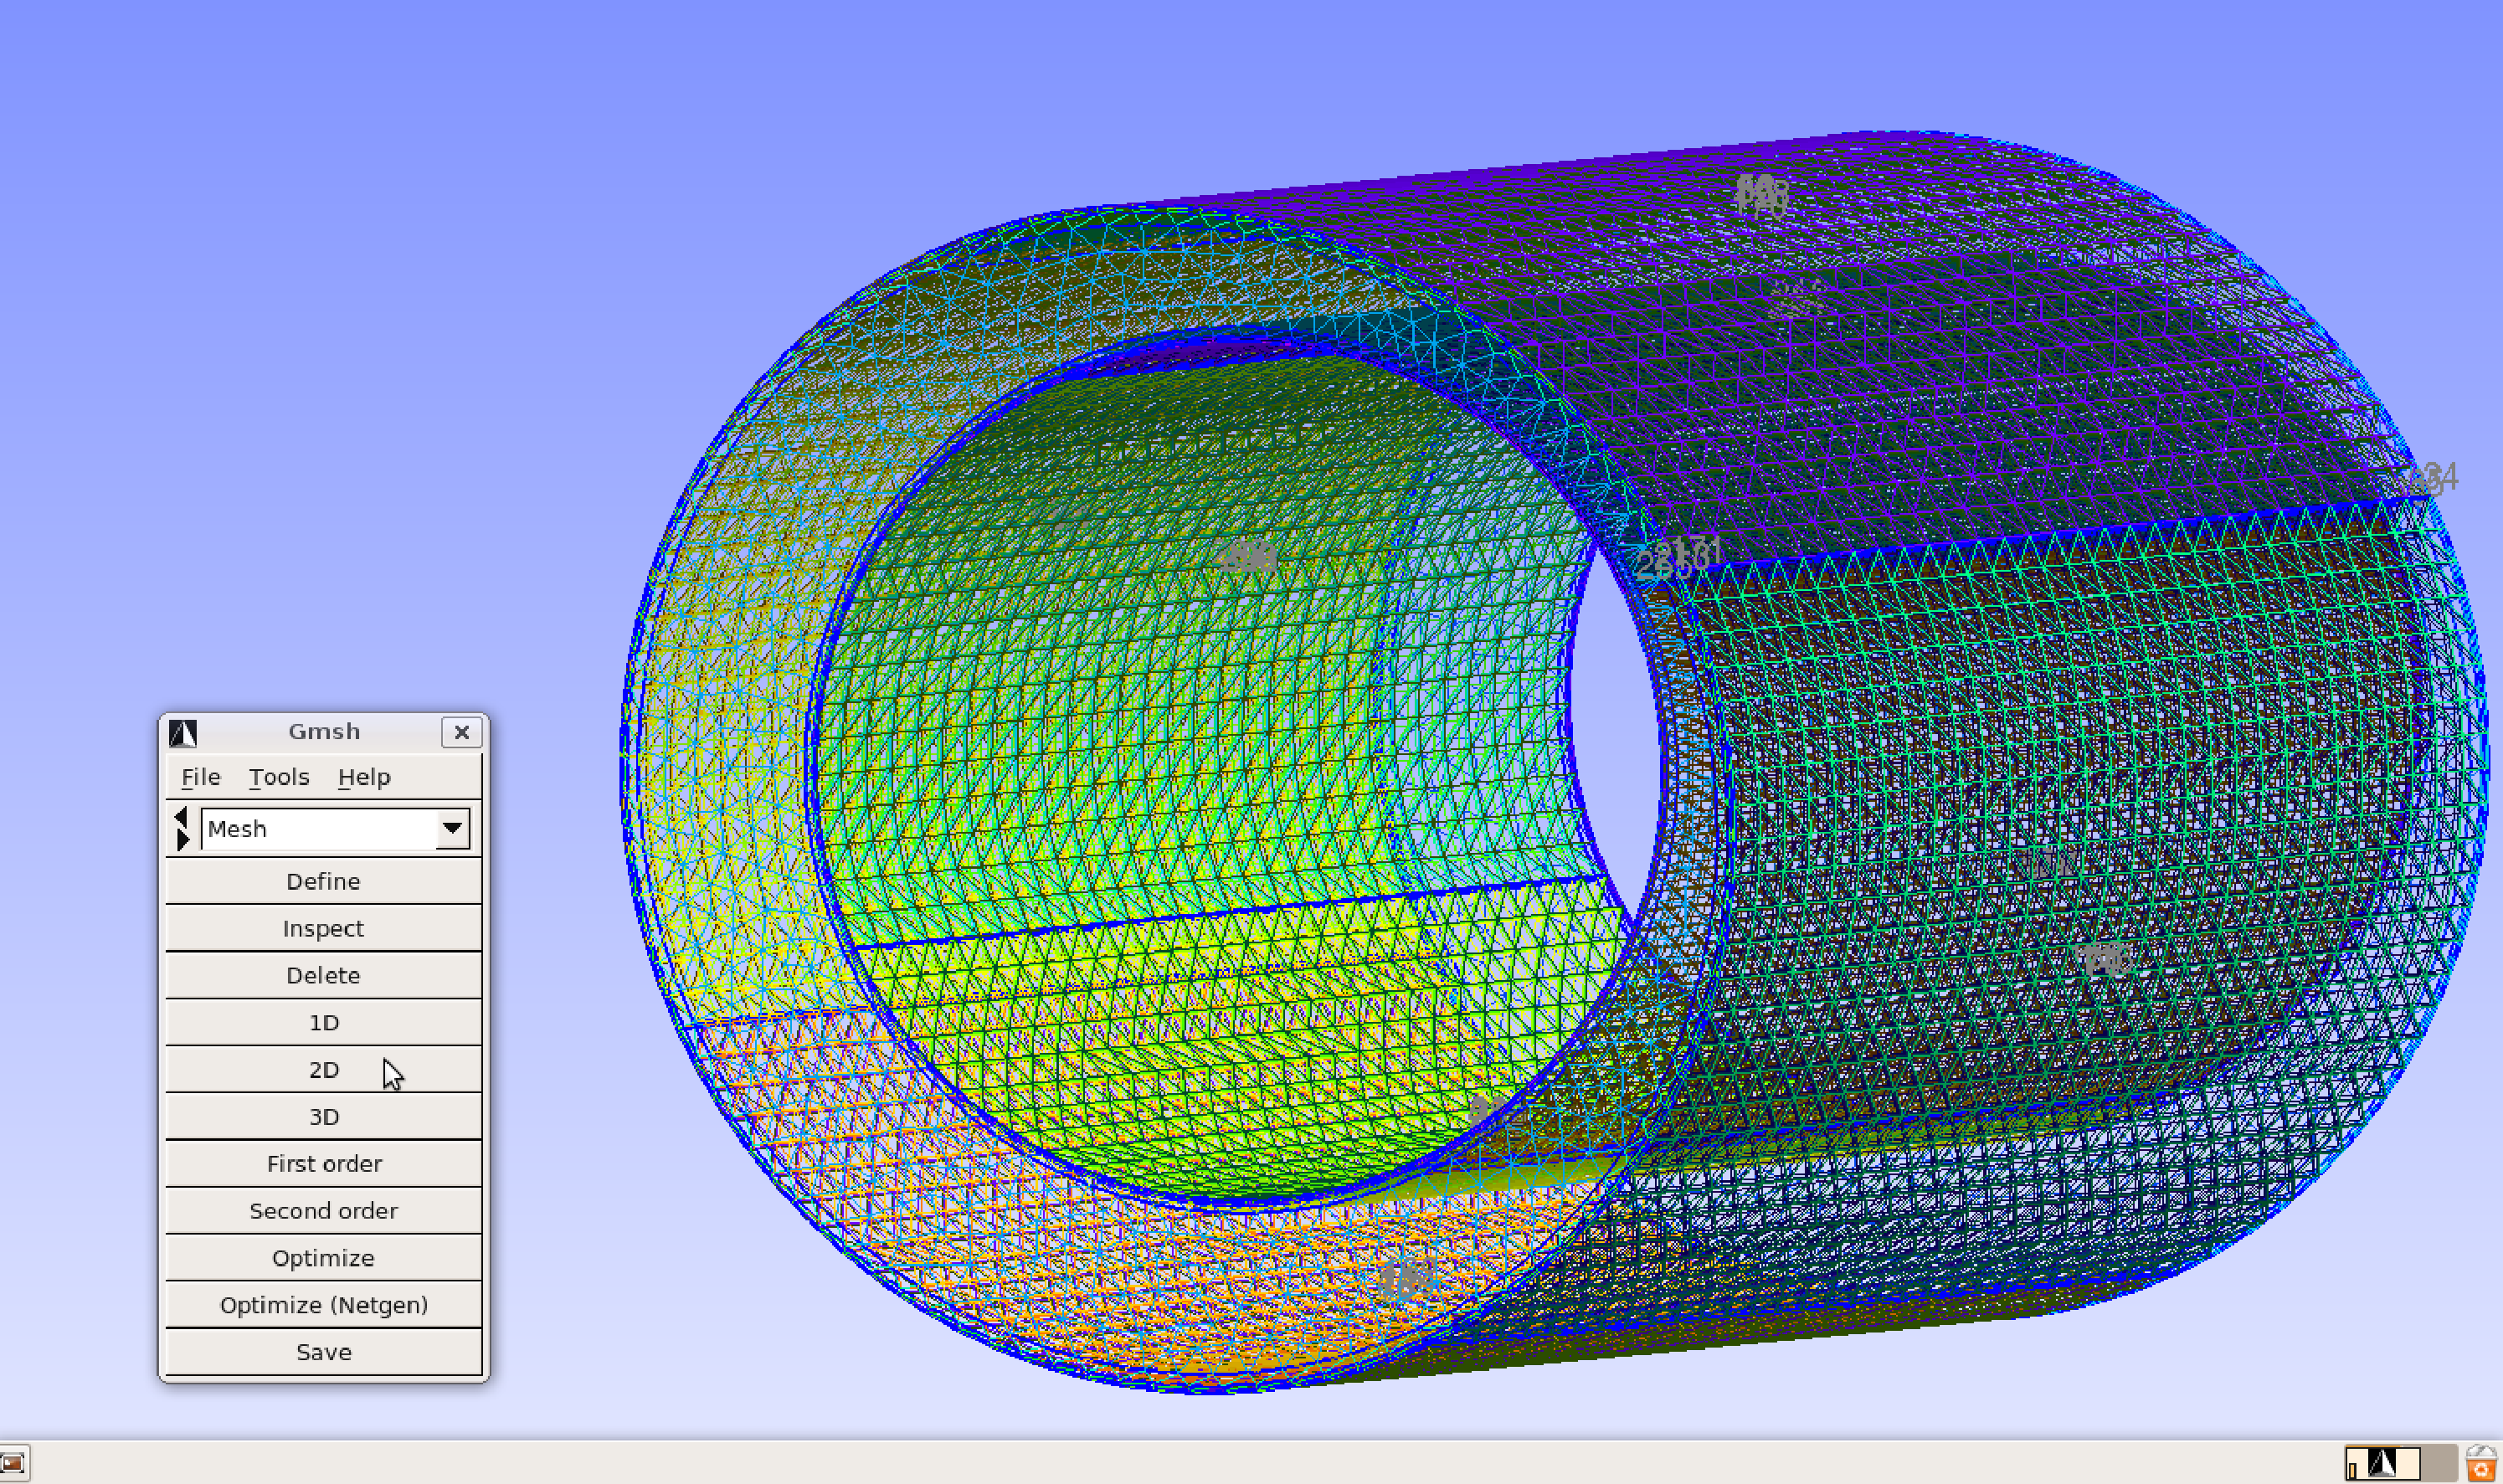
\includegraphics[width=\largefig]{chapters/hentschel/pdf/gmsh.pdf}
  \caption{The figure shows the user-interface of Gmsh during the making
    of a mesh.}
  \label{fig:Gmsh_mesh}
\end{figure}

To capture possible sharp gradients close to the boundary we introduce
a few boundary layers.  This is obtained by adding mesh layers; that
is, copies of the elliptic arcs that are gradually scaled to increase
the maximum edge length. The code example below shows the creation of
the layers close to the outer ellipse. The inner layers are created
similarly.
\begin{anycode}
outer_b1[] = Dilate {{0, 0, 0}, 1.0 - 0.1*lc } {
Duplicata{  Line{10}; Line{11}; Line{12}; Line{13}; } };
outer_b2[] = Dilate {{0, 0, 0}, 1.0 - 0.3*lc } {
Duplicata{  Line{10}; Line{11}; Line{12}; Line{13}; } };
outer_b3[] = Dilate {{0, 0, 0}, 1.0 - 0.8*lc } {
Duplicata{  Line{10}; Line{11}; Line{12}; Line{13}; } };
\end{anycode}
Here the command \emp{Duplicata} copies the expressions, while \emp{Dilate} scales them.
The single arcs are dilated separately since the arc points are necessary for further treatment. Remember that no arcs with angles smaller than $\pi$ are allowed. Again we need a representation for the complete ellipses defined by line loops, as
\begin{anycode}
Line Loop(22) = {outer_b1[]};
\end{anycode}
that are necessary to define the surfaces between all neighboring ellipses similar to:
\begin{anycode}
Plane Surface(32) = {20,22};
\end{anycode}
Finally, all surfaces are listed in the Extrude command.

The test meshes of 1.75 cm seemed to have a fully developed region
around the mid-cross sections, right where we want to observe the flow
profile. Testing different numbers of tubular layers for the length of
1.75, 2.5 and 5 cm showed that the above mentioned observations of
wave-like structures occurred less for longer pipes, even though the
number of layers was low compared to the pipe length.  The presented
results were simulated on meshes of length 5 cm with 30 layers in
z-direction and three layers on the side boundaries. The complete code
can be found in \emp{csf/mesh\_generation/gmsh}.

\subsection{Example 1: simulation of a pulse in the SAS}

In the first example we represent the spinal cord and the surrounding dura mater as two straight non-concentric cylinders, created using Gmsh.
The simulation results for an appropriate mesh can be found in
Figure~\ref{fig:case1}. The plots show the velocity component in tubular direction
at the mid-cross section of the model. The flow profiles are taken at
the time steps of maximum flow in both directions and during the
transition from systole to diastole. For maximal systole, the
velocities have two peak rings, one close to the outer, the other
close to the inner boundary. We can see sharp profiles at the maxima
and bidirectional flow at the local minimum during diastole.

\begin{figure}
\bwfig
  \ffigbox{\caption{The case with a circular cord and the boundary
      condition based on the pressure pulse in the
      heart~\citep{SmithChase2ShawEtAl2006}. The pictures show the
      velocity in z-direction for the non-symmetric pulse at the time
      steps $t=0.07s, 0.18s, 0.25s$. Notice that we use different
      color scales for the different time steps. The same color scales
      will be used in all subsequent figures.}\label{fig:case1}}
          {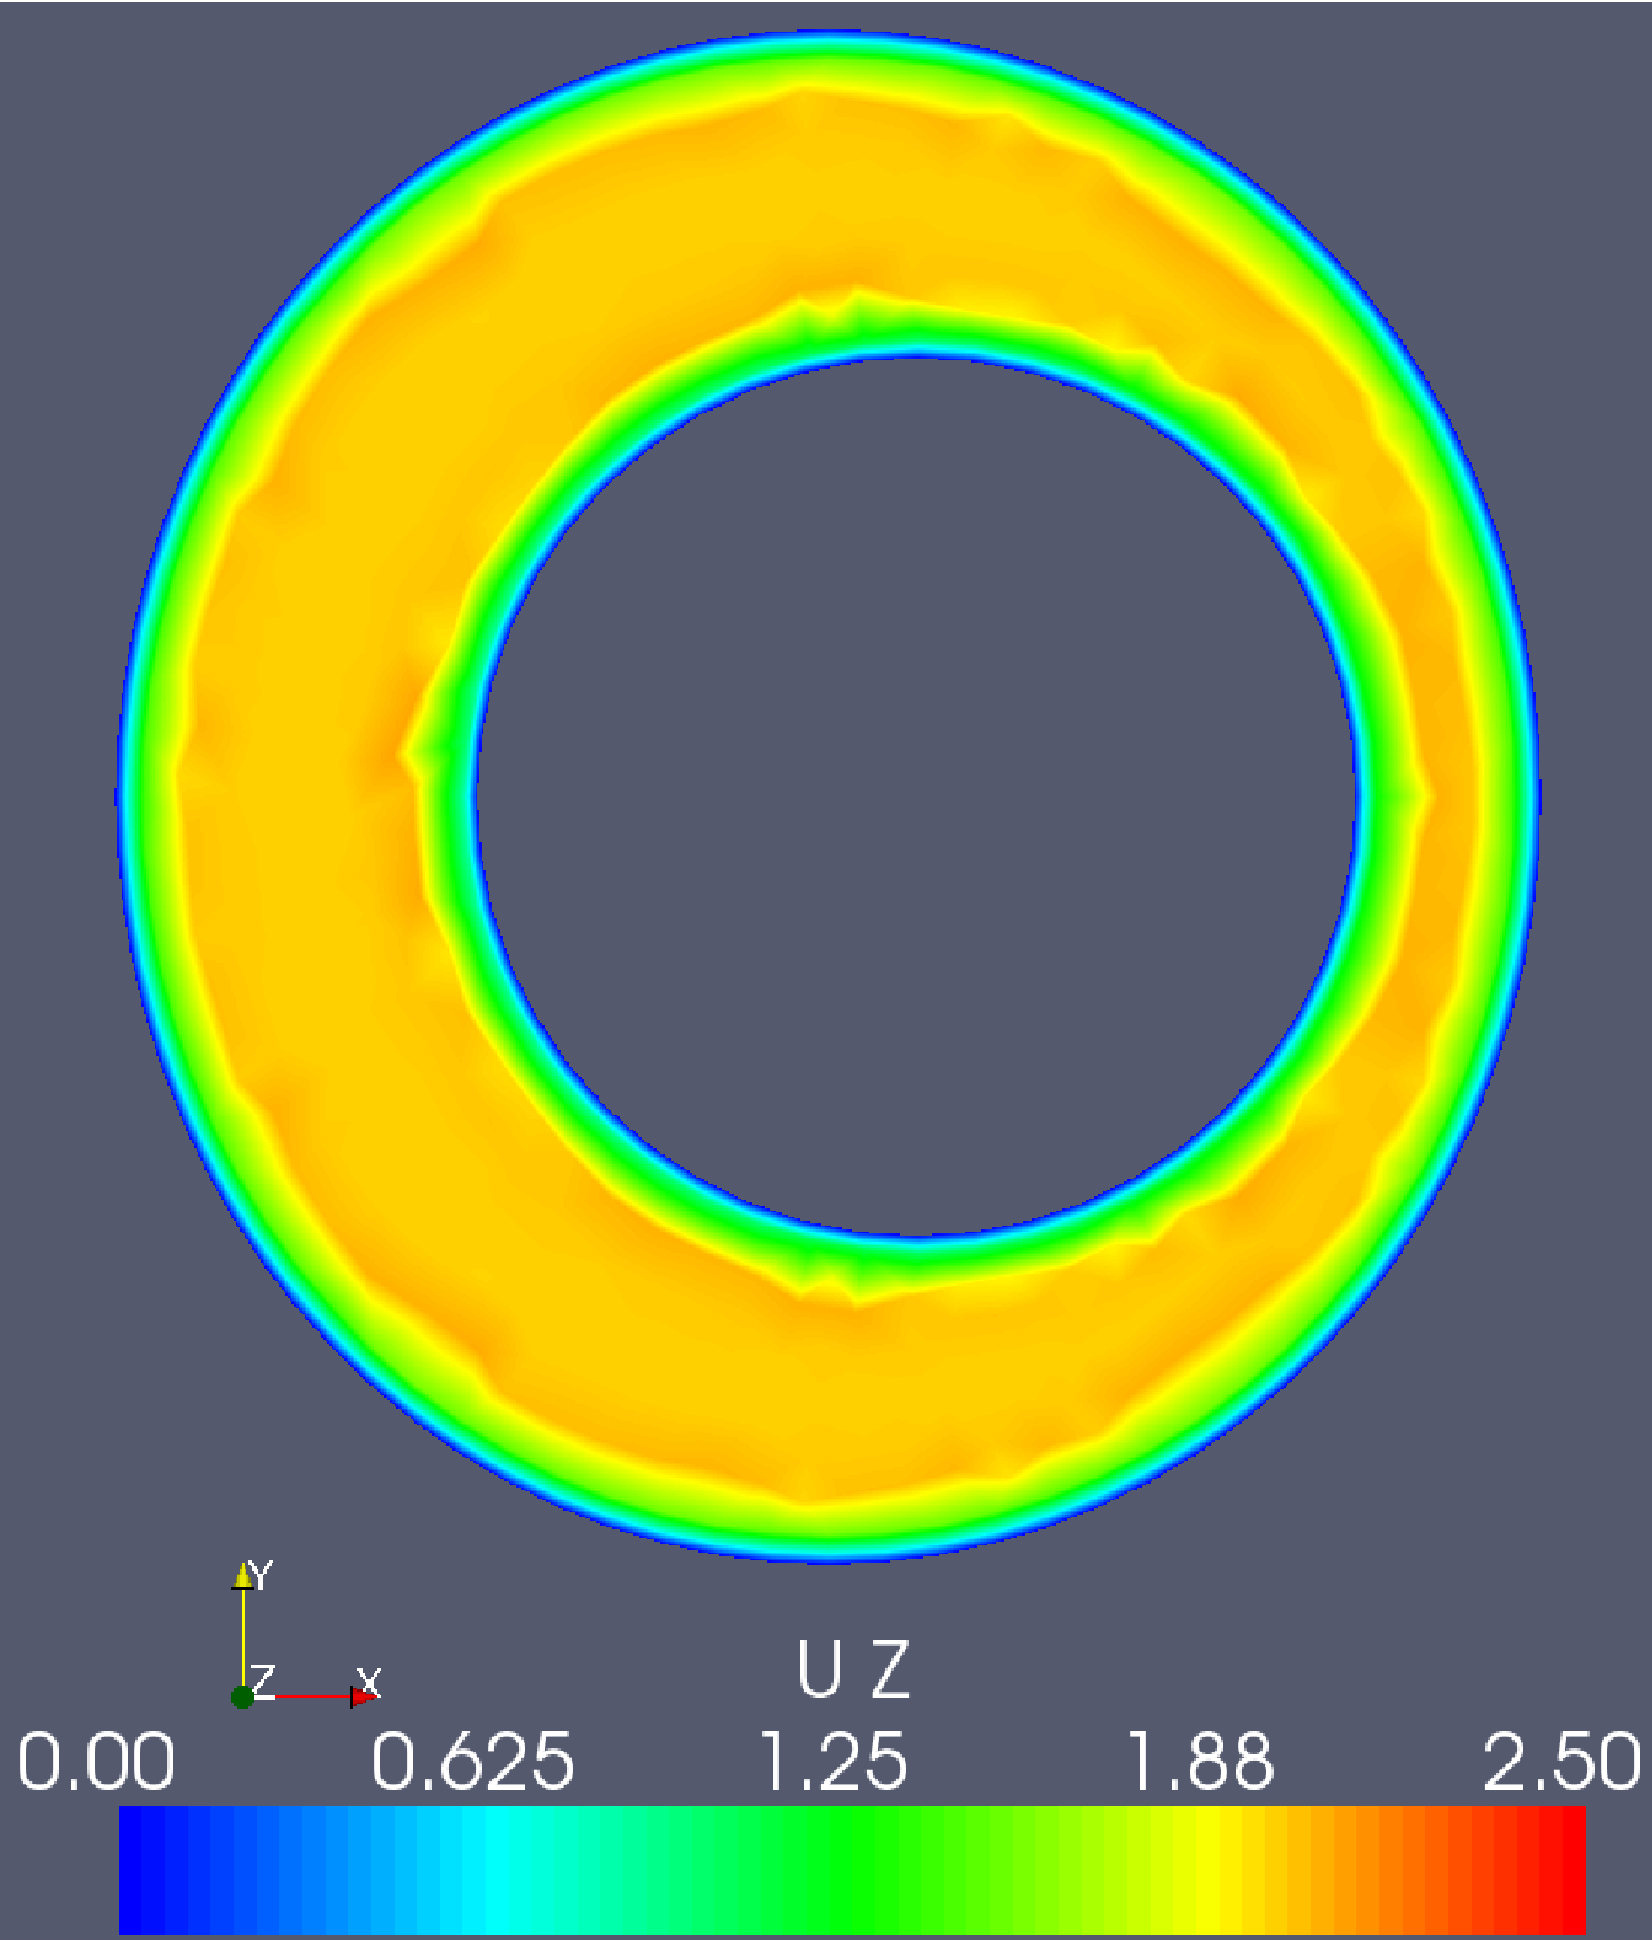
\includegraphics[width=\threefigsfull]{chapters/hentschel/pdf/pulse_f1_08_sysmax_nmb7.pdf}
           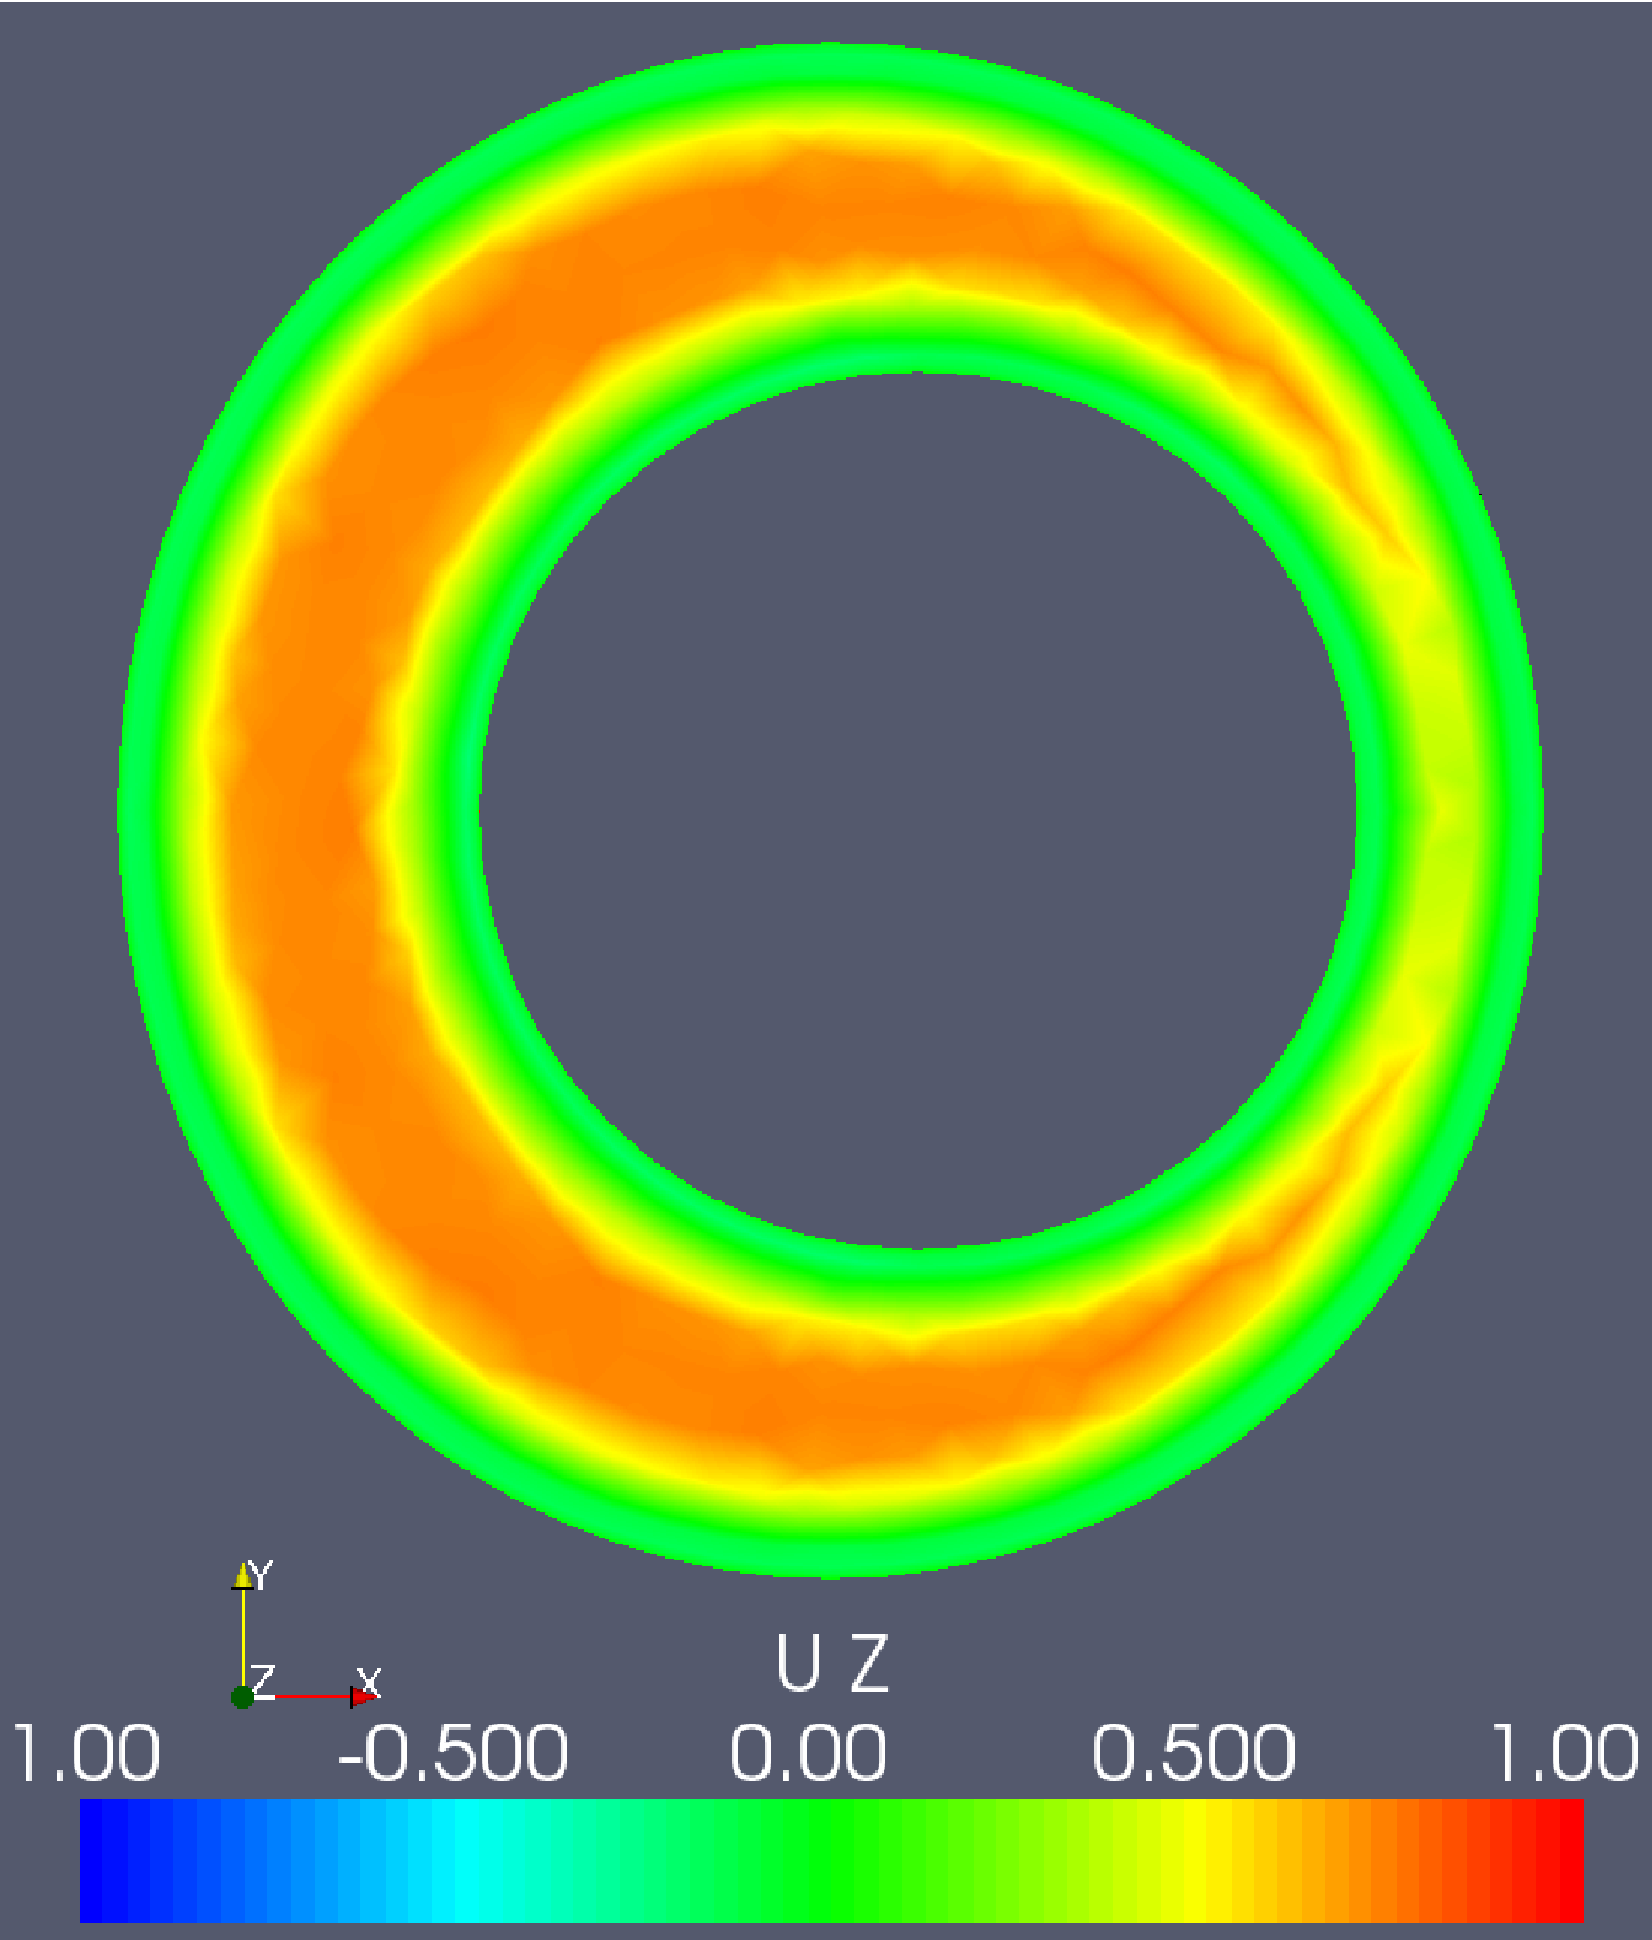
\includegraphics[width=\threefigsfull]{chapters/hentschel/pdf/pulse_f1_08_sysdia_nmb18.pdf}
           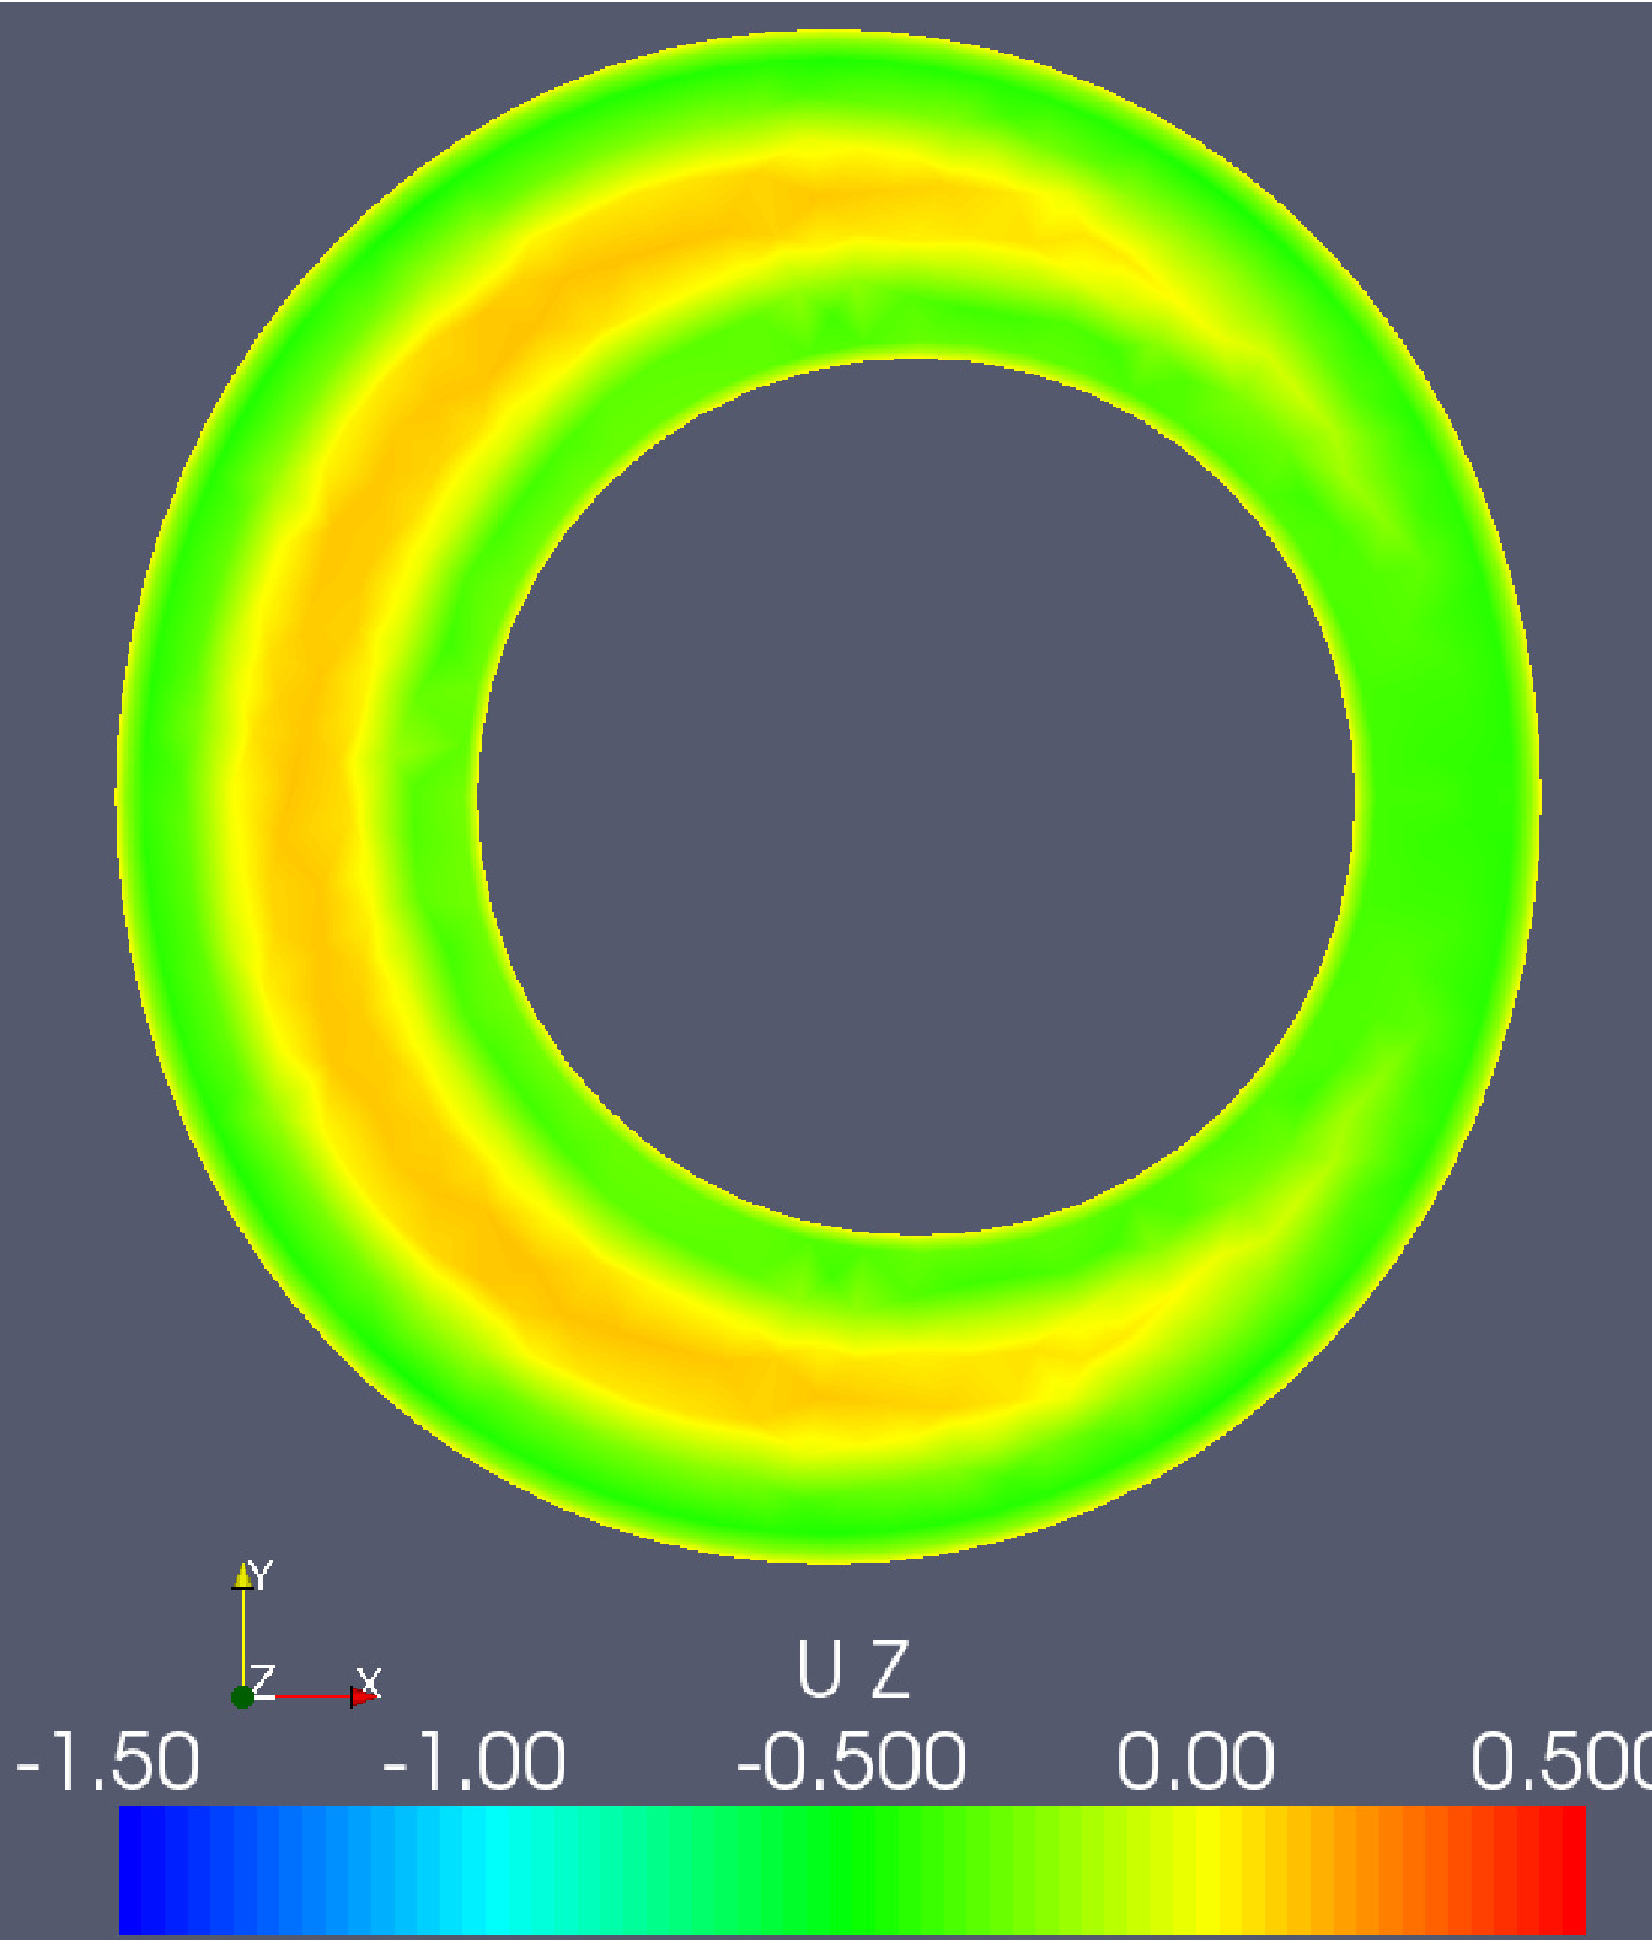
\includegraphics[width=\threefigsfull]{chapters/hentschel/pdf/pulse_f1_08_diamin1_nmb25.pdf}}
\end{figure}

The cysts usually develop several centimeters below the Chiari I
malformation. It is therefore of interest to quantify how far pressure
and velocity instabilities can travel under realistic conditions.  To
create pressure and velocity instabilities, we assign time-dependent
but flat inlet and outlet velocity conditions on the previously
described geometry and investigate how far these instabilities travel
with the flow. We also compare three different solvers, namely the
Chorin, IPCS, and G2 schemes.  All schemes do, however, use first
order elements for both velocity and pressure. In
Table~\ref{solvers:pressurediff}, we list the pressure differences at
various places along the spinal cord computed with the three different
solvers, slightly after systole. Strangely, it appears that the G2
solver requires a 30\% bigger pressure gradient between the top and
the bottom in this case. However, the G2 solver has also produced some
peculiar results in Chapter~\ref{chap:kvs-1}. We also remark that G2
was about 15 times slower than Chorin and IPCS. Our main interest
here, however, is how far the pressure instabilities travel. All the
solvers are consistent on this point, the pressure instabilities do
not travel very far. After 1 cm, the pressure instabilities is
lessened by a factor 5-10.

\begin{table}
  \centering
  \begin{tabular}{ccccc}
    \toprule
    Pressure (Pa)\ Solver & Chorin & IPCS & G2 \\
    \midrule
    $\Delta_z p \ 5.0\,\mathrm{cm}$  & 99.6 & 101.3 & 130     \\
    $\Delta_{xy} p  \ 0.1\,\mathrm{cm}$  &  2.1 & 2.6 & 0.9     \\
    $\Delta_{xy}  p  \ 0.5\,\mathrm{cm}$  & 0.8 & 1.1 & 0.4     \\
    $\Delta_{xy}  p  \ 1.0\,\mathrm{cm}$  & 0.3 & 0.3 & 0.2     \\
    $\Delta_{xy}  p  \ 2.0\,\mathrm{cm}$  &  0.03 & 0.03 & 0.01     \\
    \bottomrule
  \end{tabular}
  \caption{Pressure differences between various places in the spinal canal.
    The first row, $\Delta_z 5.0\,\mathrm{cm}$ list the pressure difference between the
    top and bottom. The next rows list pressure differences, $\Delta_{xy}
    p$ in the cross sections $0.1\,\mathrm{cm}$, $0.5\,\mathrm{cm}$, $1.0\,\mathrm{cm}$, and $2.0\,\mathrm{cm}$ down from
    the top.}
  \label{solvers:pressurediff}
\end{table}

\subsection{Example 2: simplified boundary conditions}

Many researchers apply the sine function as inlet and outlet boundary
conditions, since its integral is zero over one period. However, its
shape is not in agreement with measurements of the cardiac flow
pulse. To see the influence of the applied boundary condition for the
defined mesh, we replaced the more realistic pulse function with a
sine, scaled to the same amount of volume transport per cardiac
cycle. The code example below implements the alternative pulse
function in the object function \emp{boundary\_conditions}. The
variable \emp{sin\_integration\_factor} describes the integral of the
first half of a sine.
\begin{python}
self.HR = 1.16 # heart rate in beats per second; from 70 bpm
self.HR_inv = 1.0/self.HR
self.SV = 0.27
self.A1 = self.area(1)
self.flow_per_unit_area = self.volume_flow/self.A1
sin_integration_factor = 0.315
self.v_max = self.flow_per_unit_area/sin_integration_factor
\end{python}
As before, we have a global function returning the sine as an object:
\begin{python}
def get_sine_input_function(V, z_index, HR, HR_inv, v_max):
    v_z = "sin(2*pi*HR*fmod(t,T))*(v_max)"
    vel = ["0.0", "0.0", "0.0"]
    vel[z_index] = v_z
    defaults = {"HR":HR, "v_max":v_max, "T":HR_inv}
    sine = Expression(vel, defaults)
    return sine
\end{python}
that is called instead of \emp{get\_pulse\_input\_function} in the function \emp{boundary\_conditions}:
\begin{python}
self.g1 = get_sine_input_function(V, self.z_index, self.factor, self.A,
                                 self.HR_inv, self.HR, self.b, self.f1)
\end{python}

The pulse and the sine are sketched in
Figure~\ref{fig:sin_pulse}. Both functions are marked at the points of
interest: maximum systolic flow, around the transition from systole to
diastole and the (first, local) minimum. Results for sinusoidal
boundary conditions are shown in Figure~\ref{fig:case2} The shape of
the flow profile is similar at every time step, only the magnitudes
change. No bidirectional flow was discovered in the transition from
positive to negative flow. Compared to the results received by the
more realistic pulse function, the velocity profile generated from
sinusoidal boundaries is more homogeneous over the cross section.

\begin{figure}
\bwfig
  \ffigbox{\caption{The case with circular cord and the boundary
      condition based on a sine function. The pictures show the
      velocity in z-direction as response to a sine boundary condition
      for the time steps $t=0.2, 0.4, 0.6$.}\label{fig:case2}}
          {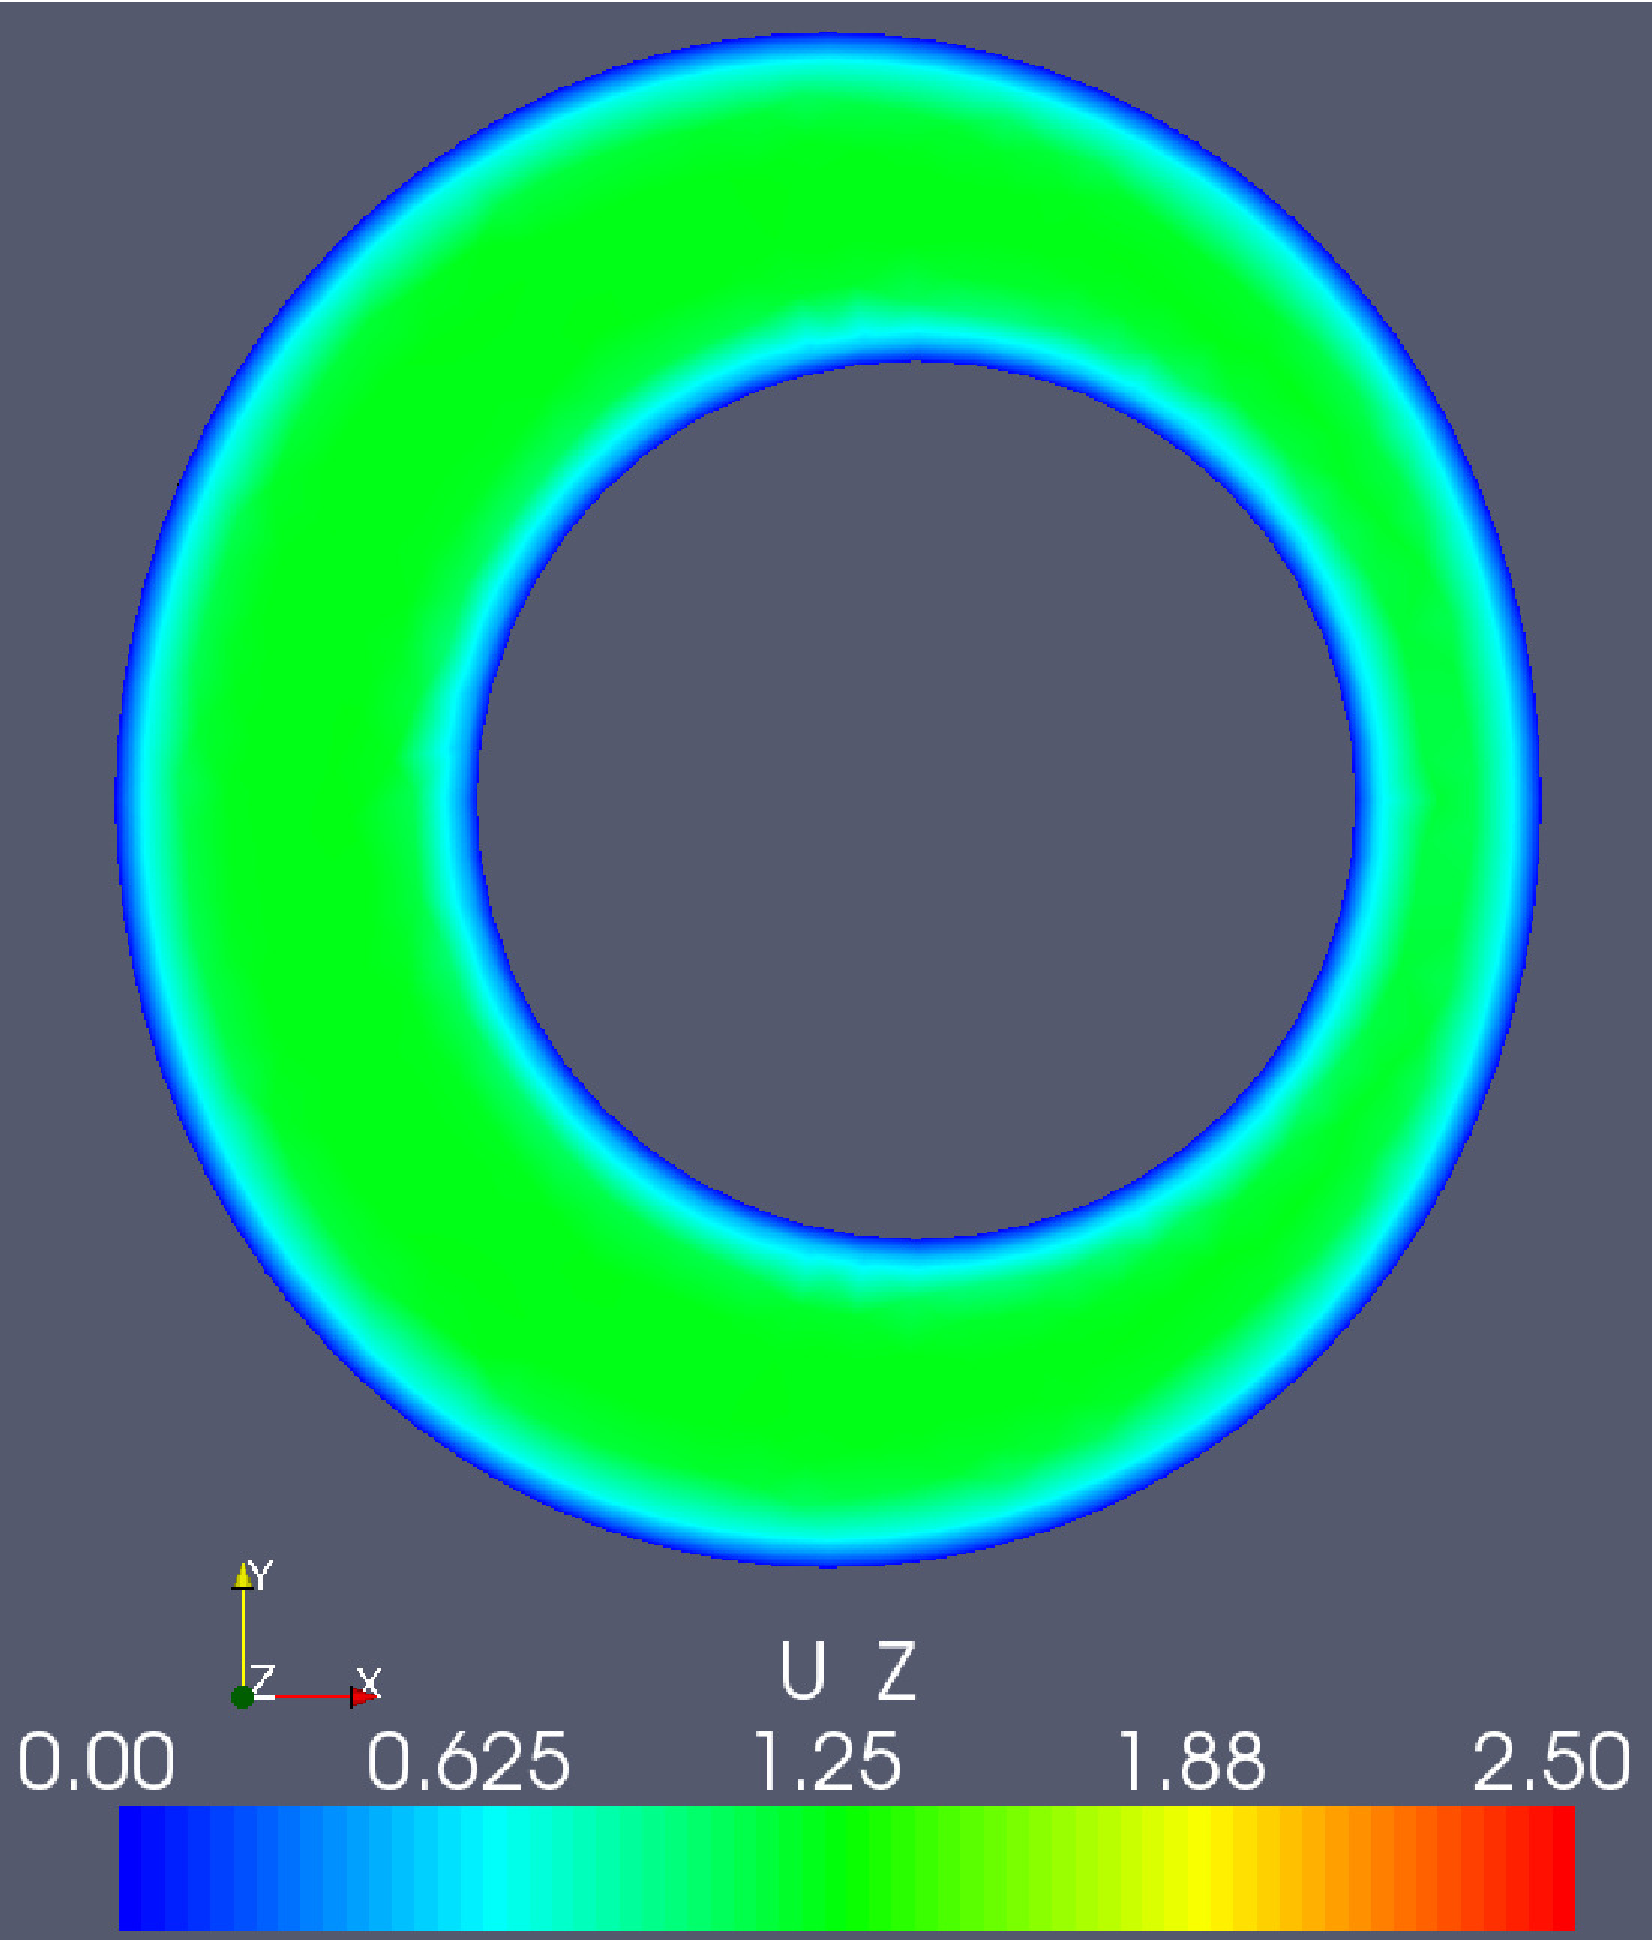
\includegraphics[width=\threefigsfull]{chapters/hentschel/pdf/sin_sysmax_nmb2.pdf}
            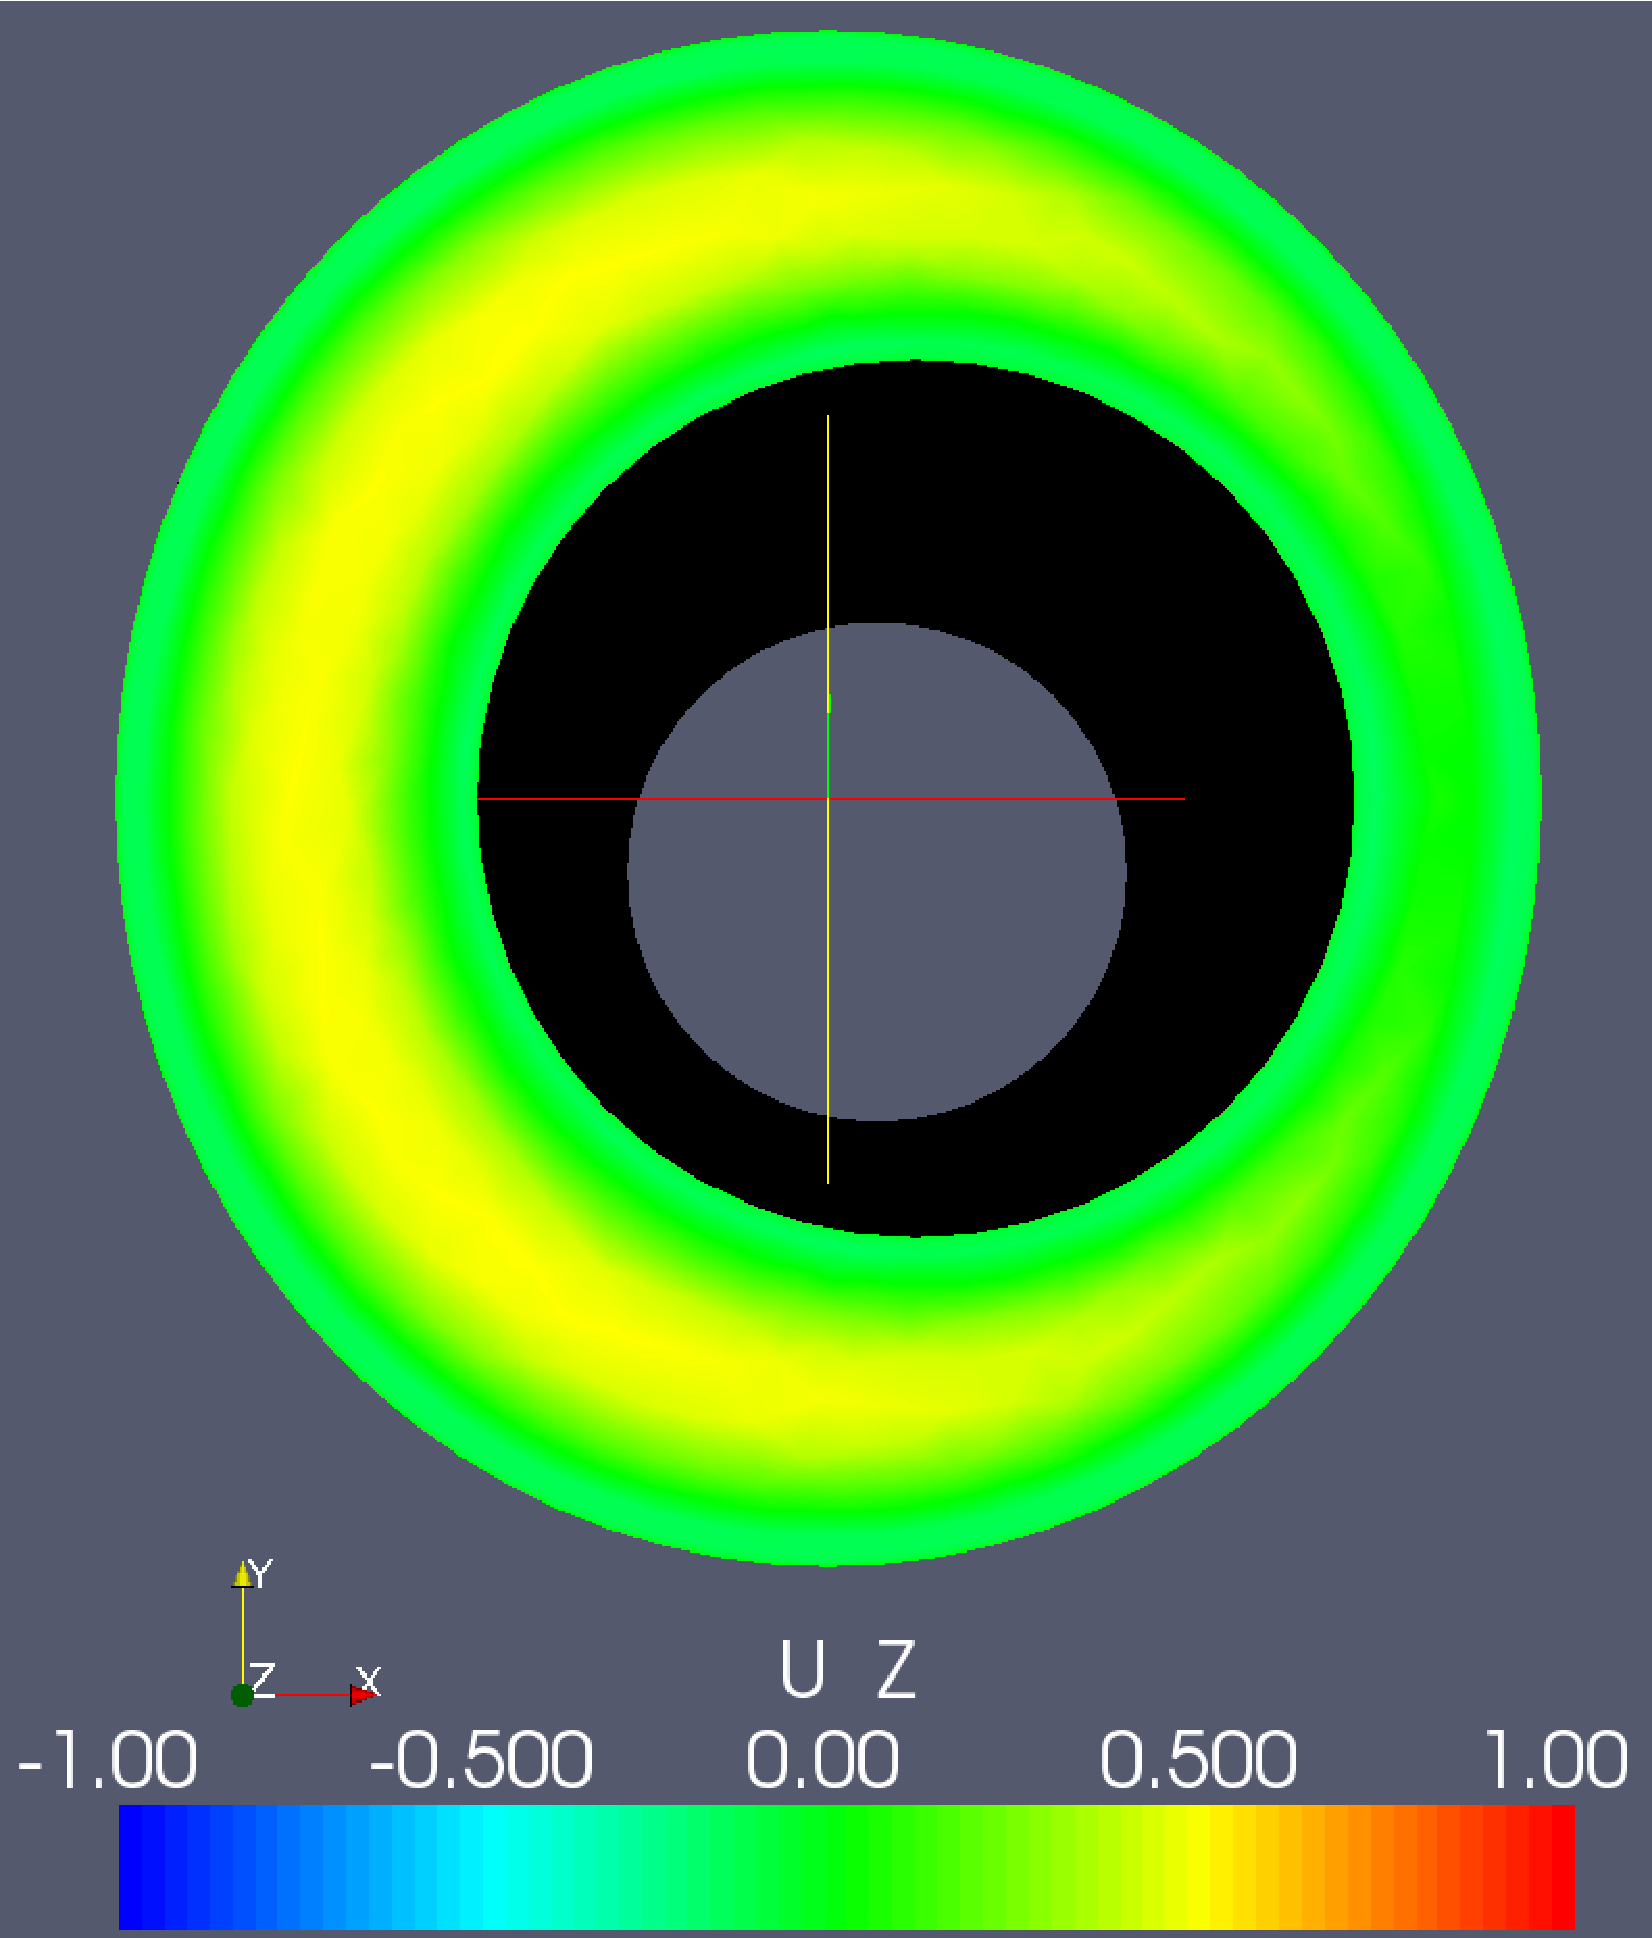
\includegraphics[width=\threefigsfull]{chapters/hentschel/pdf/sin_sysdia_nmb4.pdf}
            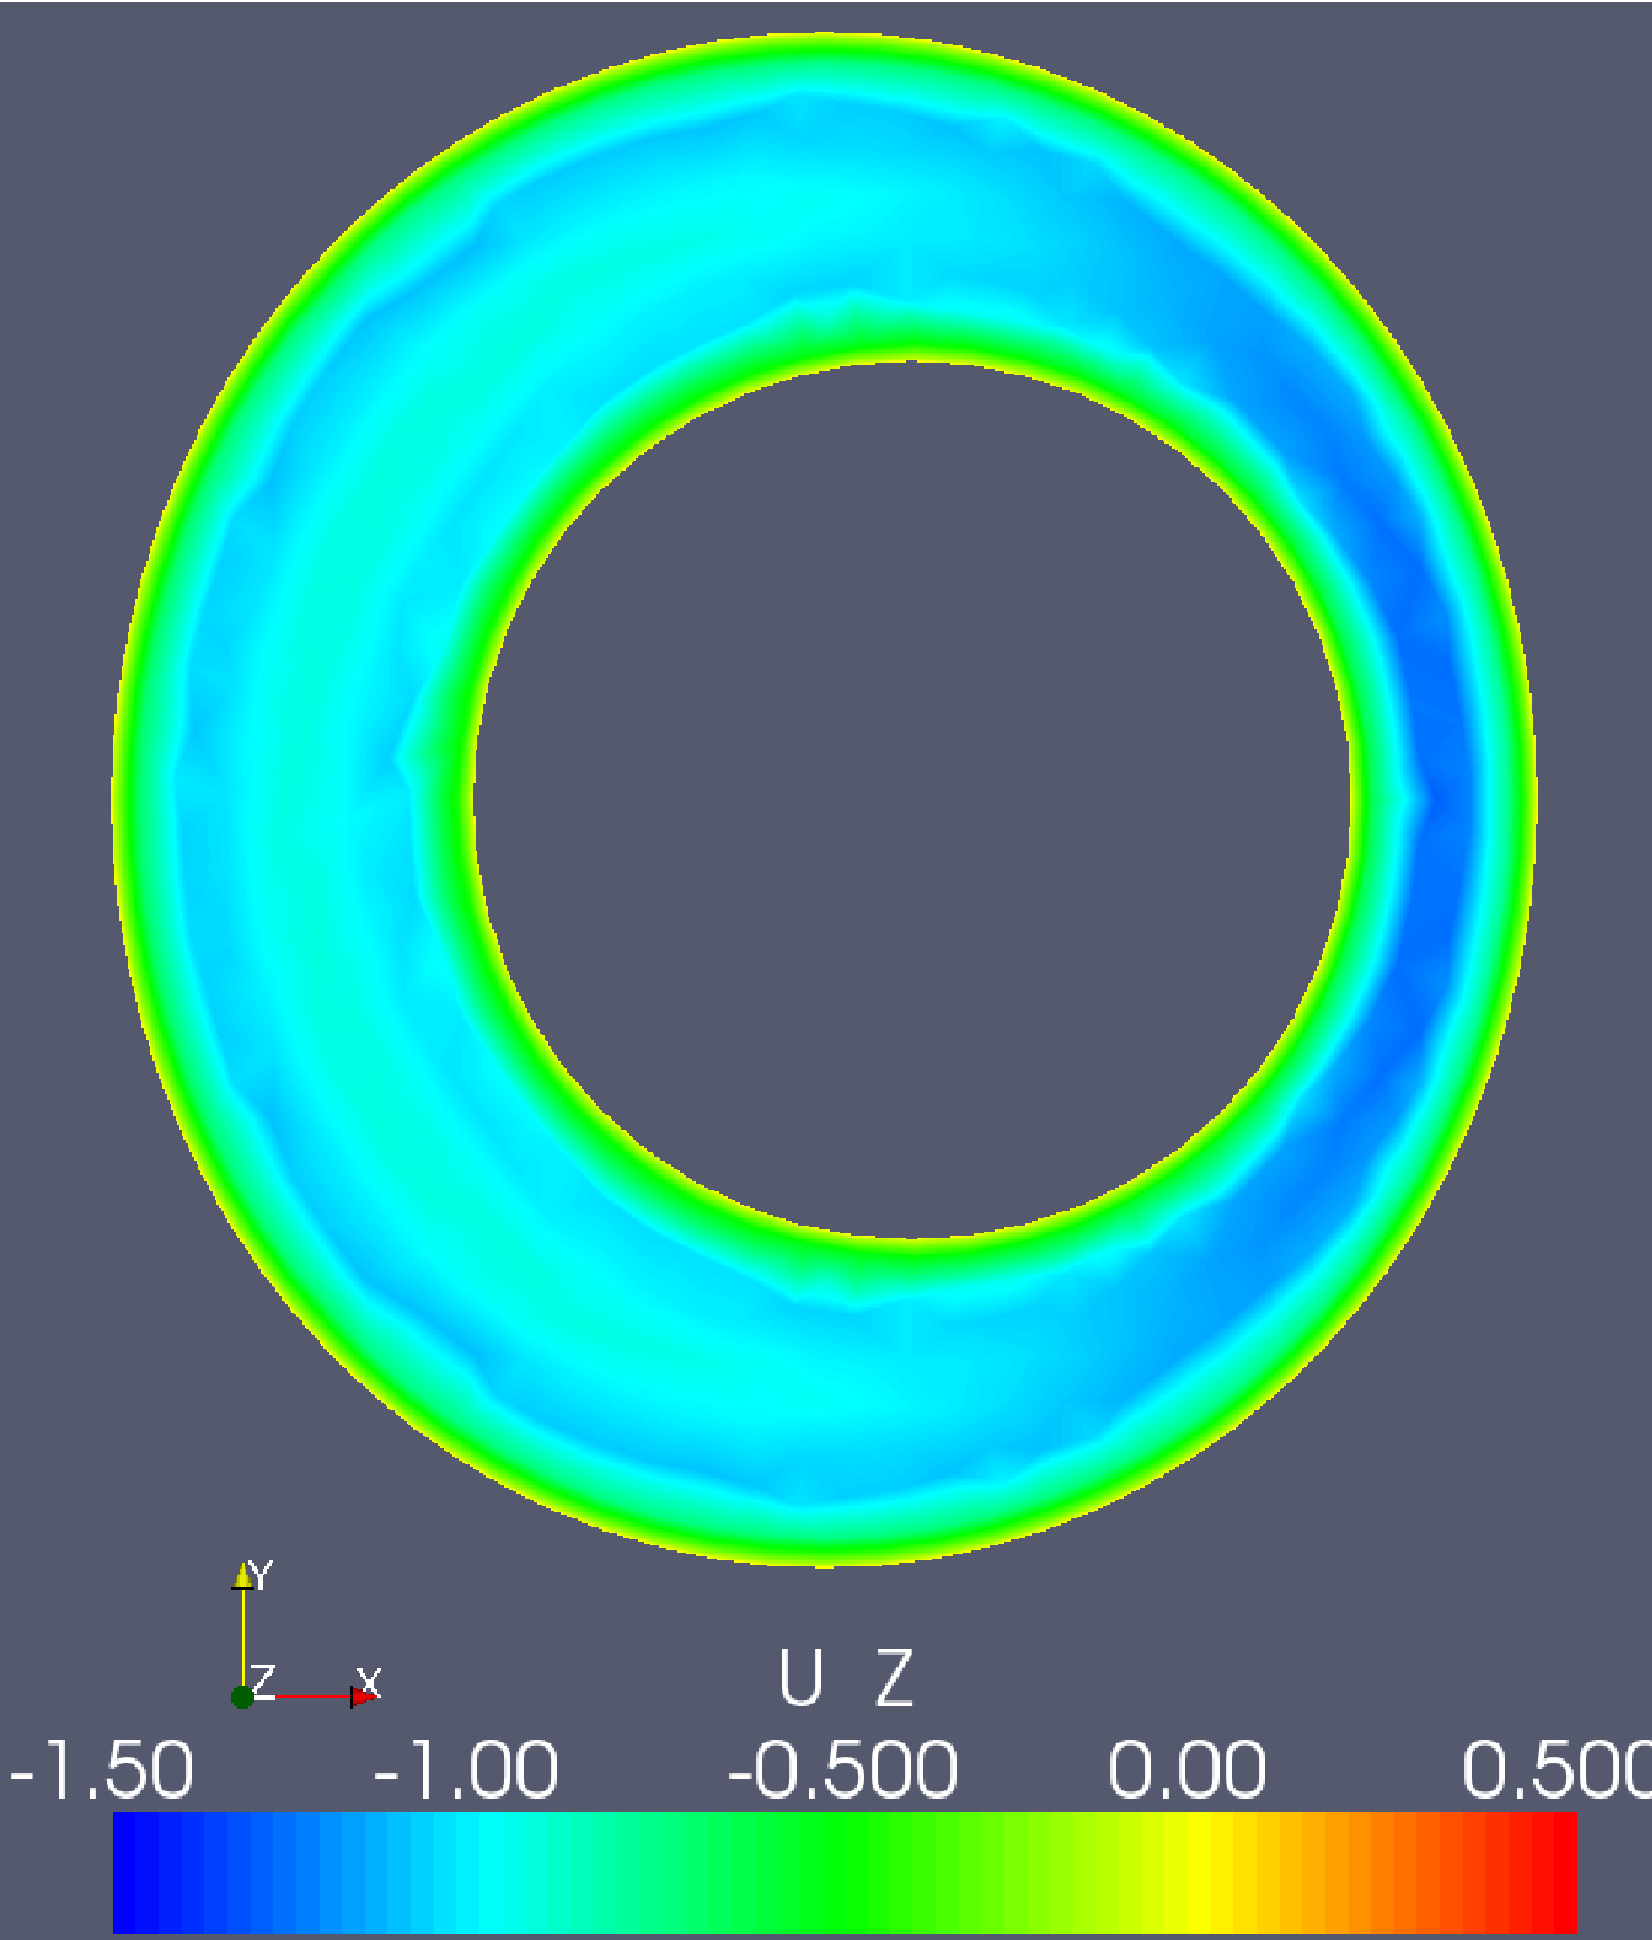
\includegraphics[width=\threefigsfull]{chapters/hentschel/pdf/sin_diamin_nmb6.pdf}}
\end{figure}

\subsection{Example 3: cord shape and position}

According to \citet{LothYardimciAlperin2001,AlperinMazdaLichtorEtAl2006},
the present flow is inertia dominated, meaning that the shape of the
cross section should not influence the pressure gradient. Changing the
length of vectors describing the ellipse from
\begin{anycode}
c = 0.4;
d = 0.4;
\end{anycode}
to
\begin{anycode}
c = 0.32;
d = 0.5;
\end{anycode}
transforms the cross section of the inner cylinder to an elliptic
shape with preserved area. The simulation results are collected in
Figure~\ref{fig:case3}. The geometry differences between the two cases
gave different flow profiles but no differences in the pressure
gradient.

A further perturbation of the SAS cross sections was achieved by
changing the displacement of the elliptic cord center from
\begin{anycode}
move = 0.08;
\end{anycode}
to
\begin{anycode}
move = 0.16;
\end{anycode}
Also for this case the pressure field was identical, with some
variations in the flow profiles, see Figure~\ref{fig:case3b}.

\begin{figure}
\bwfig
  \ffigbox{\caption{The case with an elliptic cord and the boundary
      condition based on the pressure pulse in the heart. The pictures
      show the velocity in z-direction for the non-symmetric pulse at
      the time steps $t=0.07s, 0.18s, 0.25s$.}\label{fig:case3}}
          {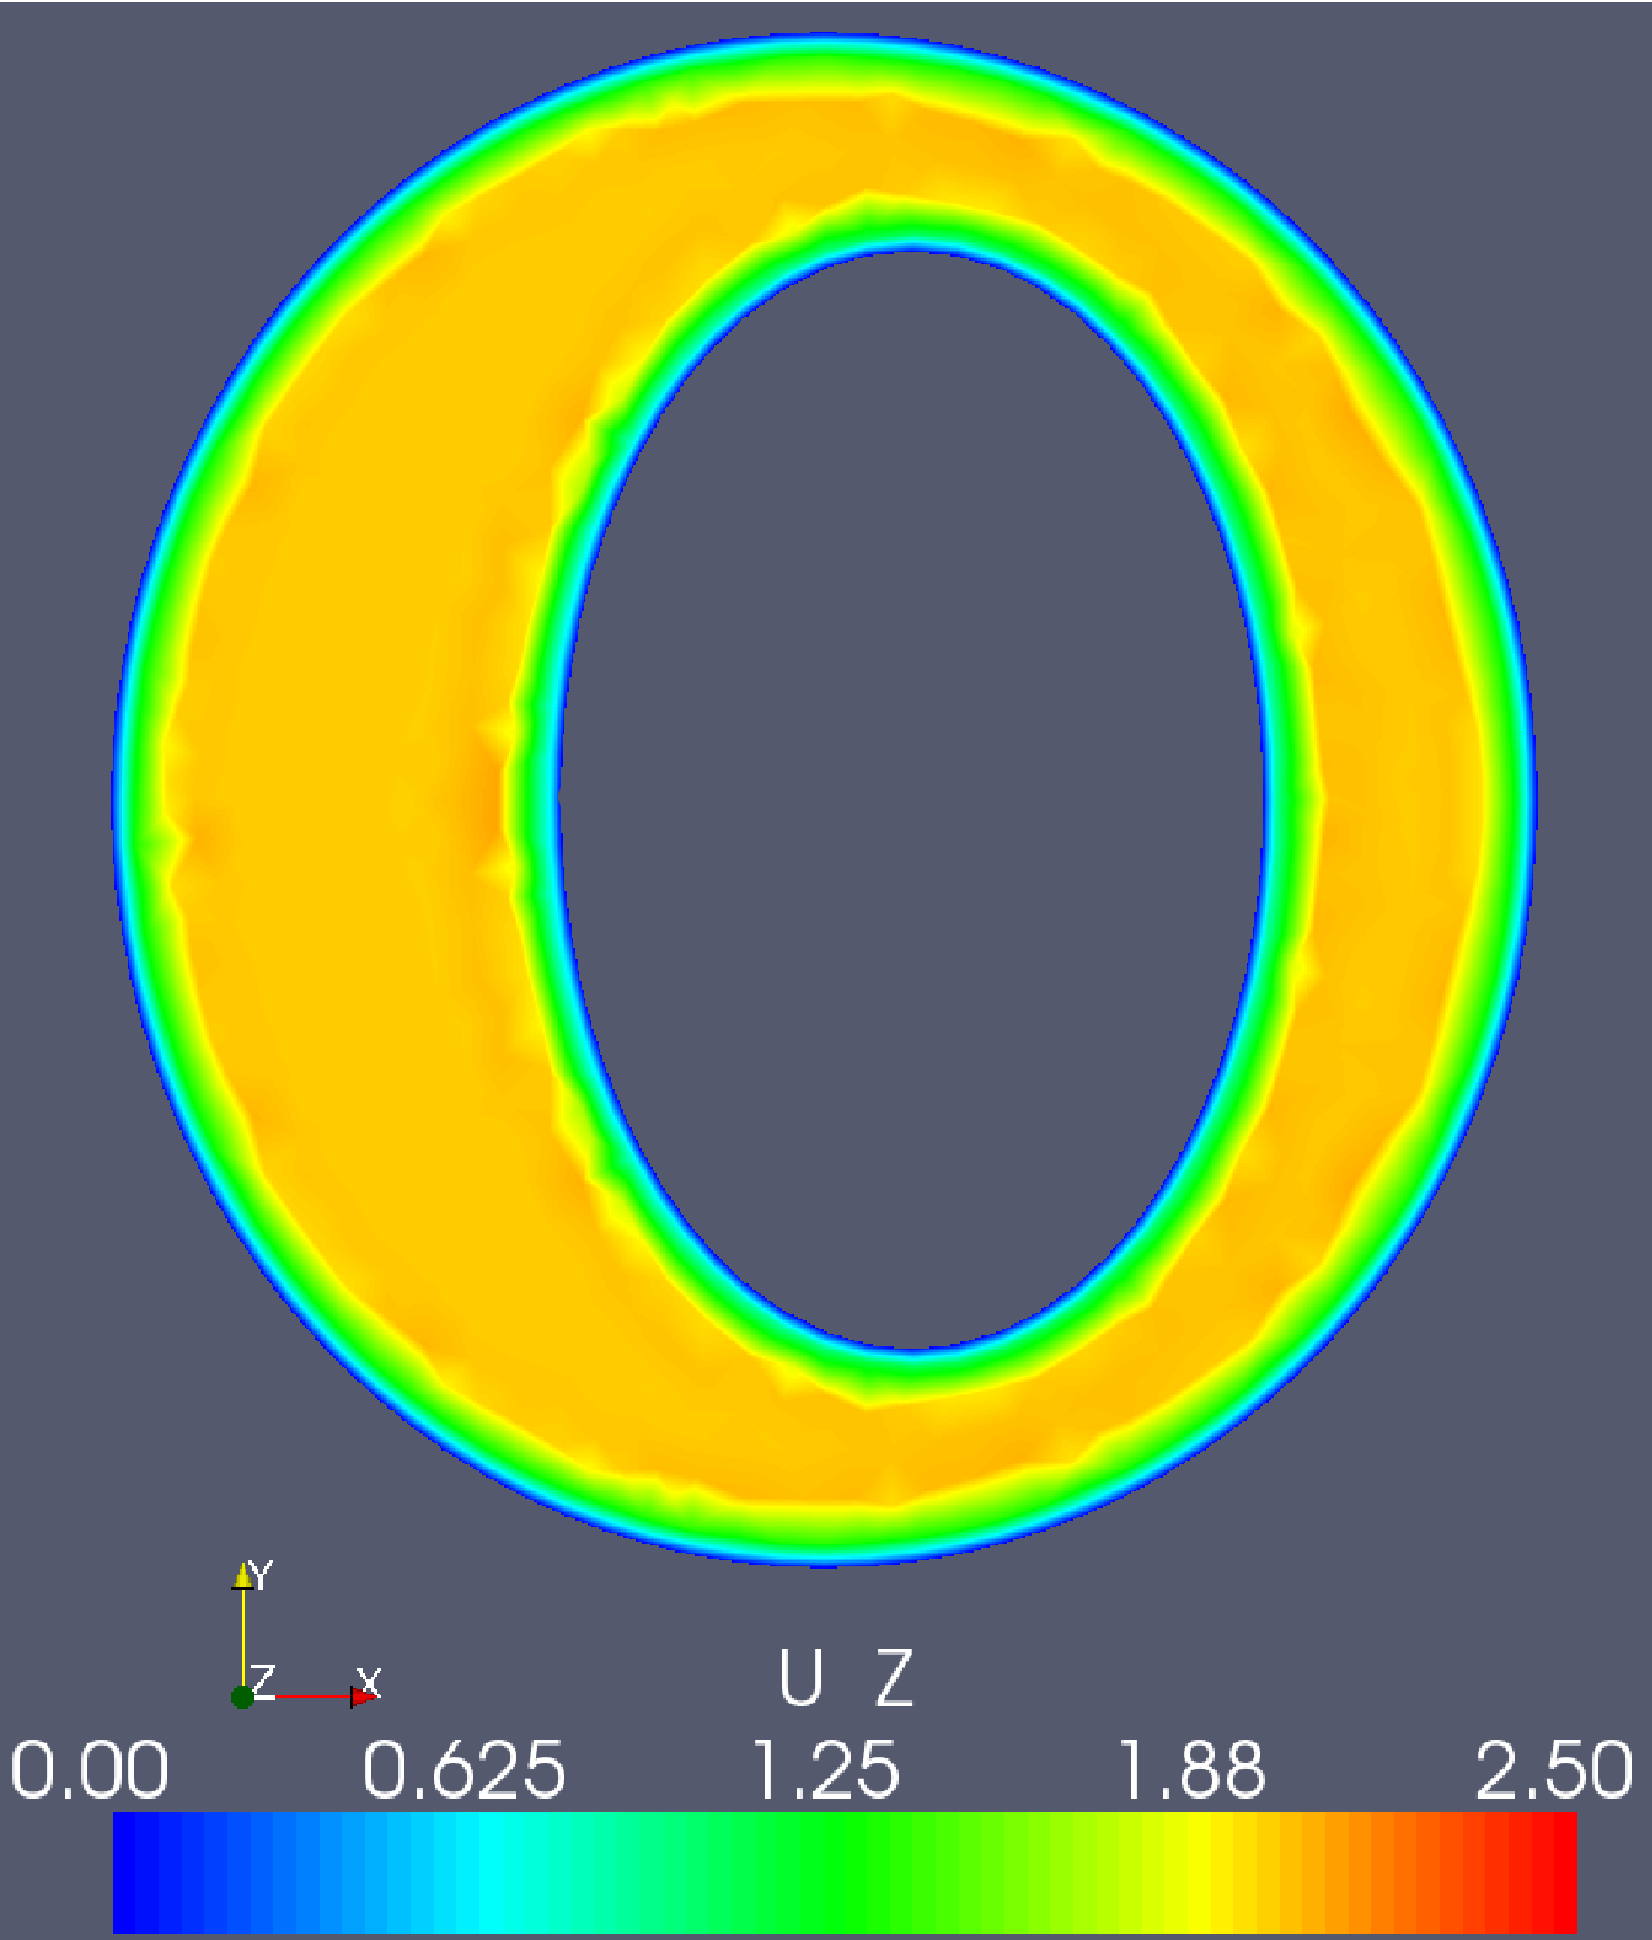
\includegraphics[width=\threefigsfull]{chapters/hentschel/pdf/pulse_f1_08_elliptic_sysmax_nmb7.pdf}
            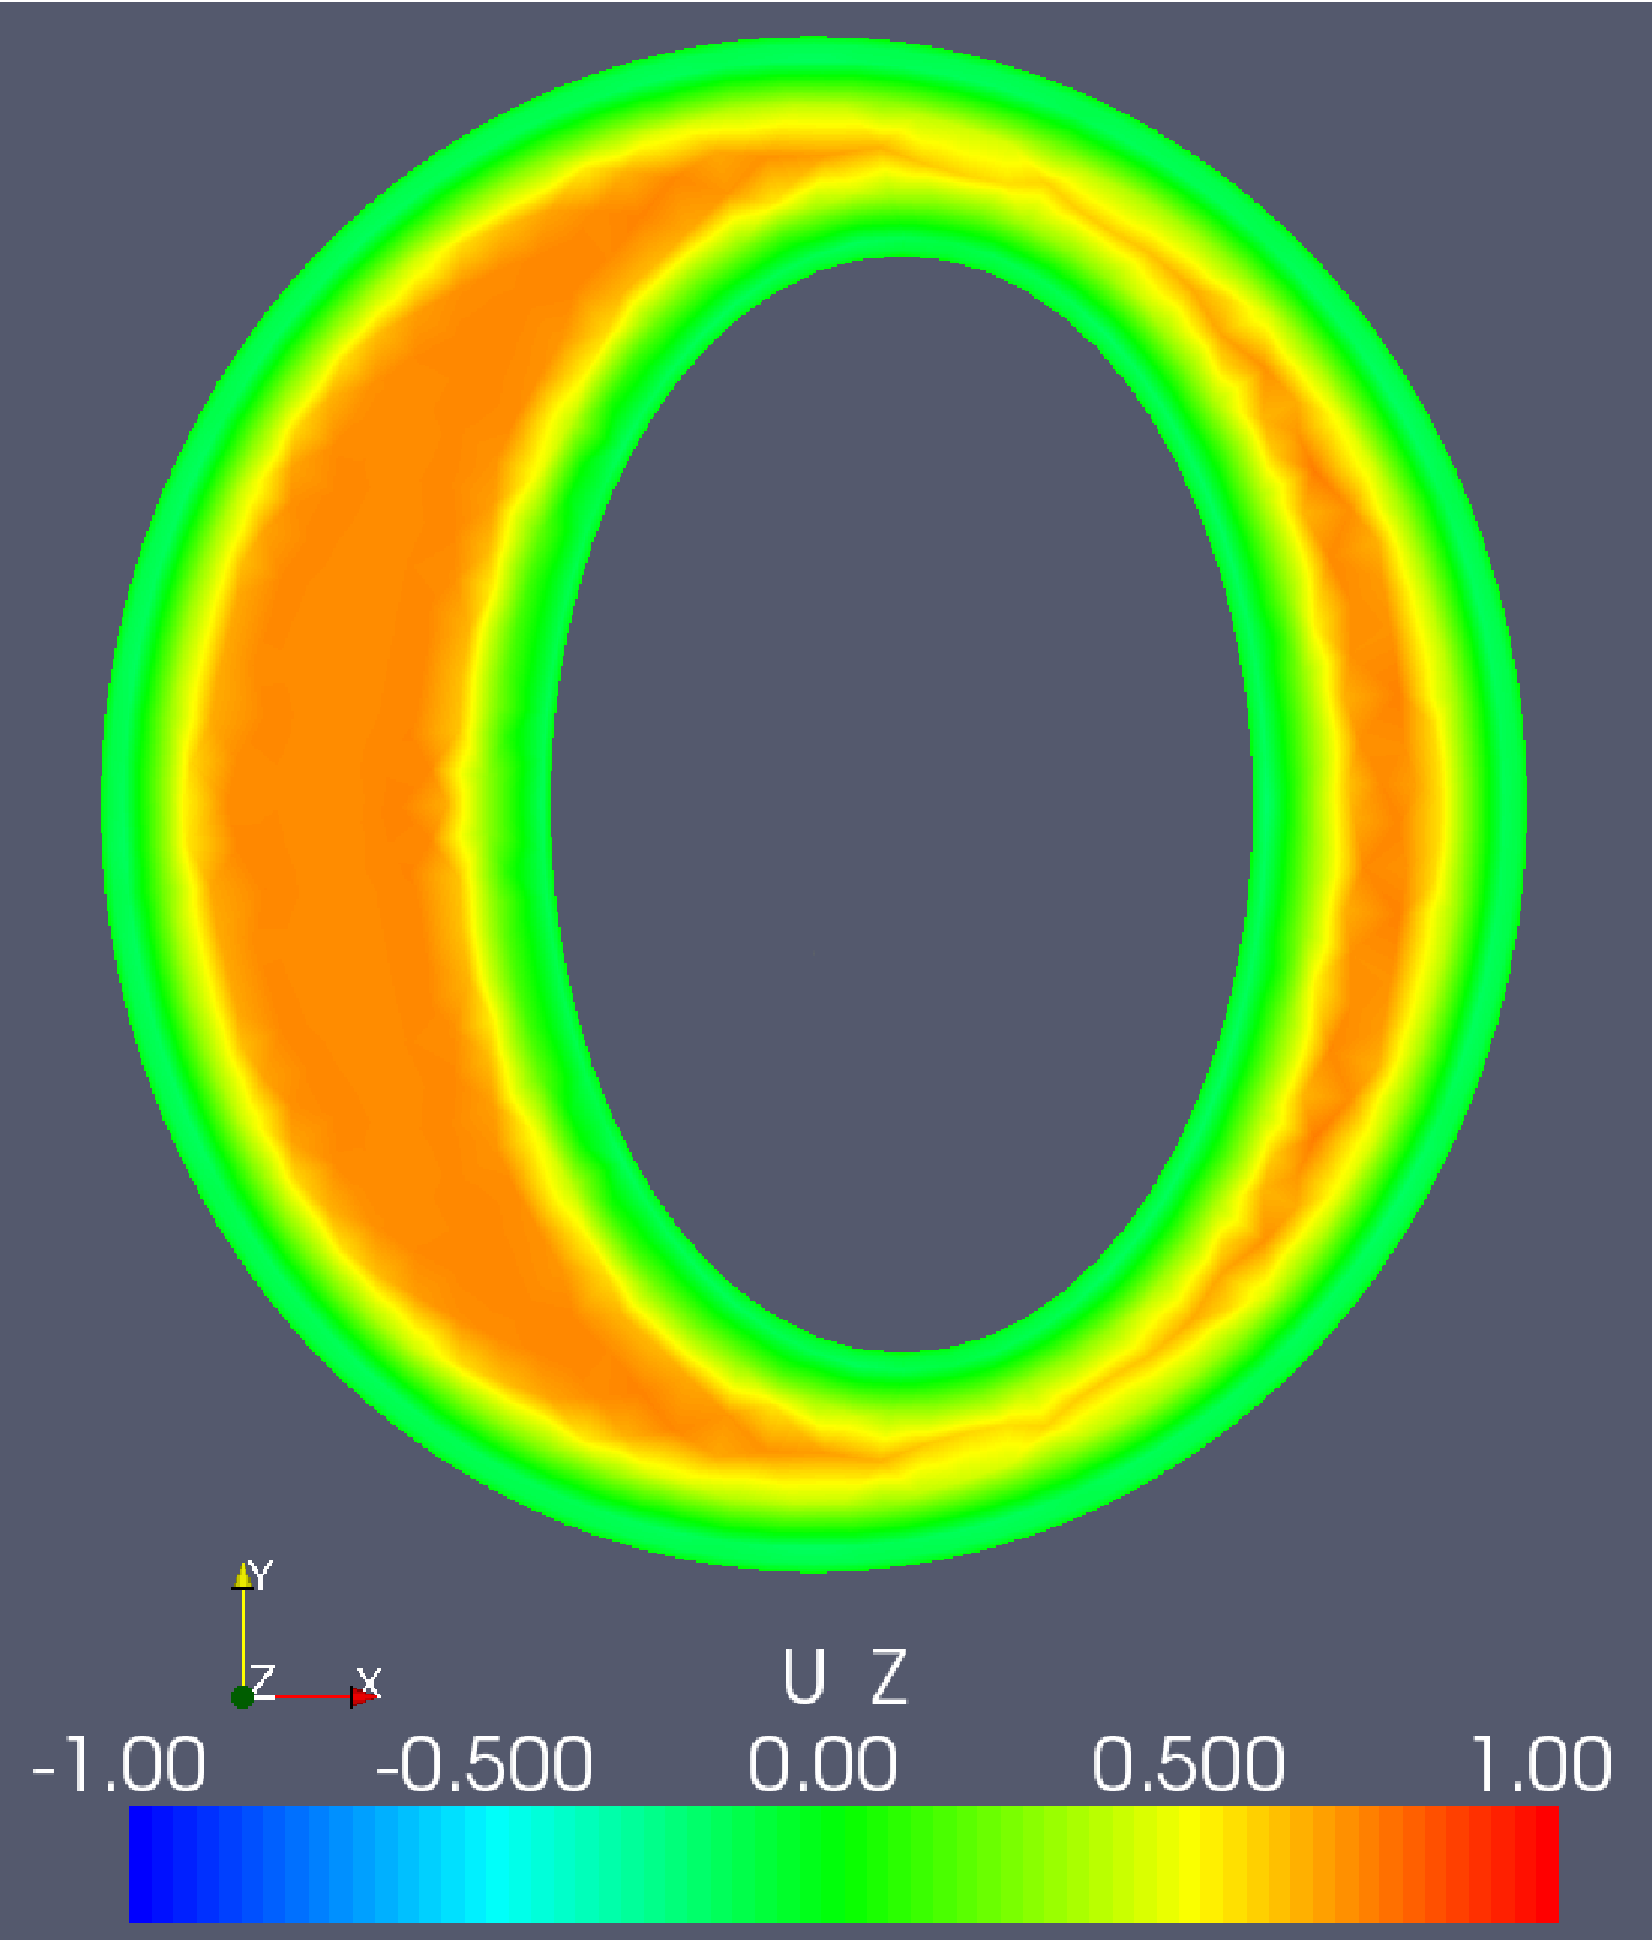
\includegraphics[width=\threefigsfull]{chapters/hentschel/pdf/pulse_f1_08_elliptic_sysdia_nmb18.pdf}
            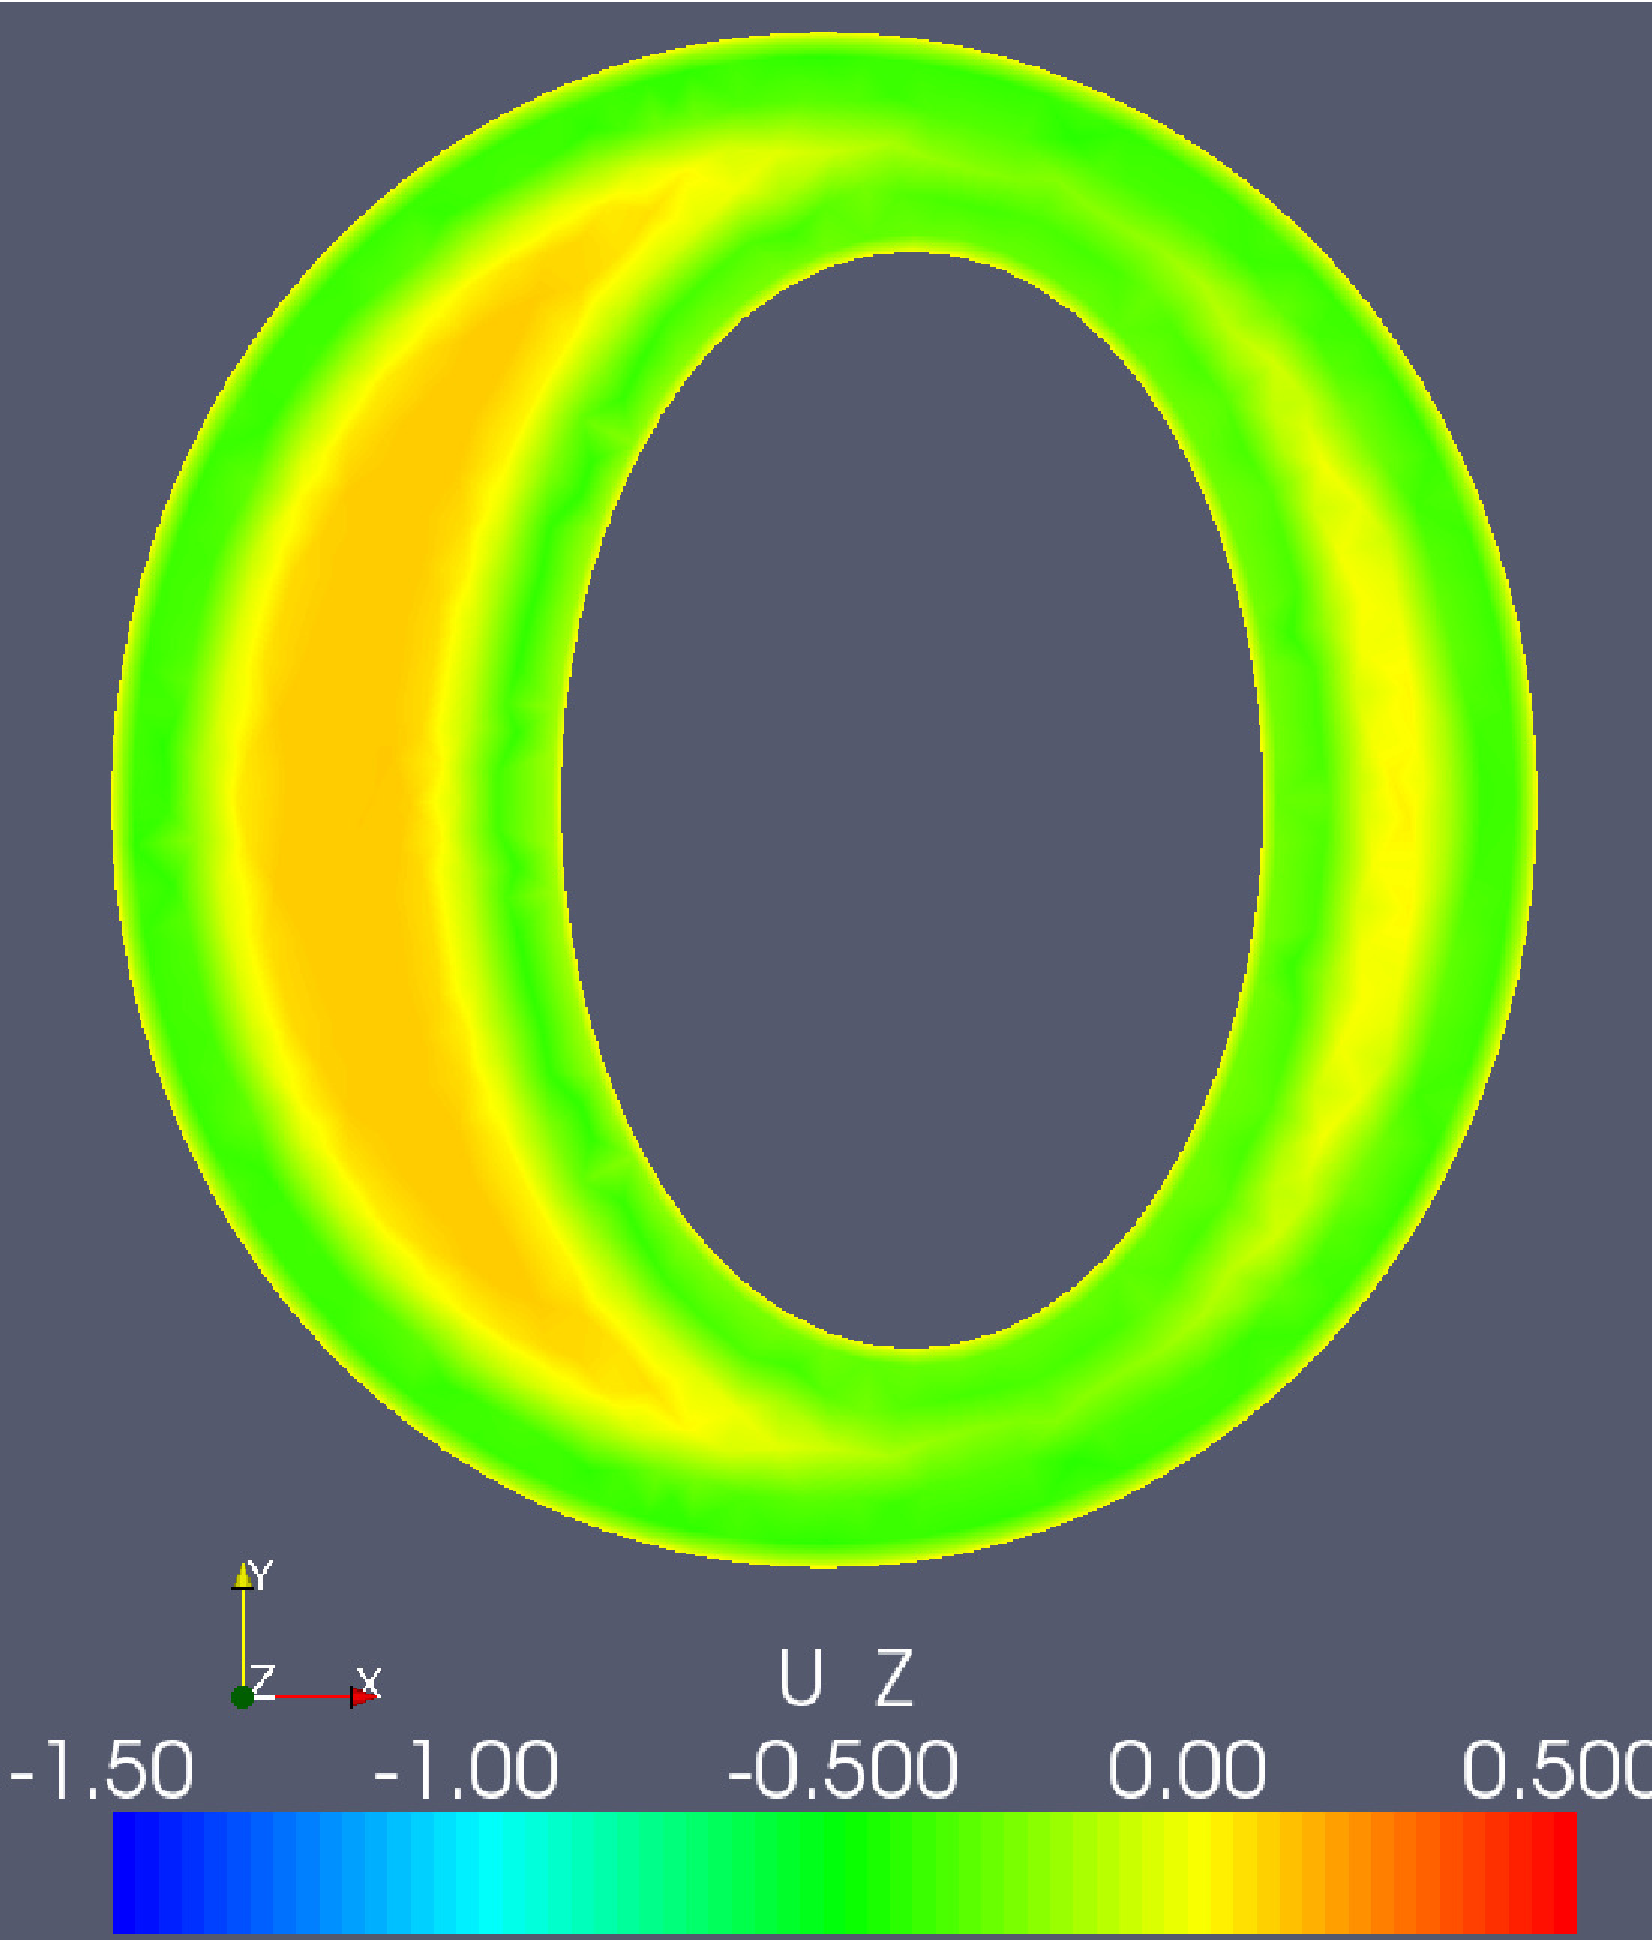
\includegraphics[width=\threefigsfull]{chapters/hentschel/pdf/pulse_f1_08_elliptic_diamin1_nmb25.pdf}}
\end{figure}

\begin{figure}
\bwfig
  \ffigbox{\caption{The case with a translated elliptic cord. The
      pictures show the velocity in z-direction for the non-symmetric
      pulse at the time steps $t=0.07s, 0.18s,
      0.25s$.}\label{fig:case3b}}
          {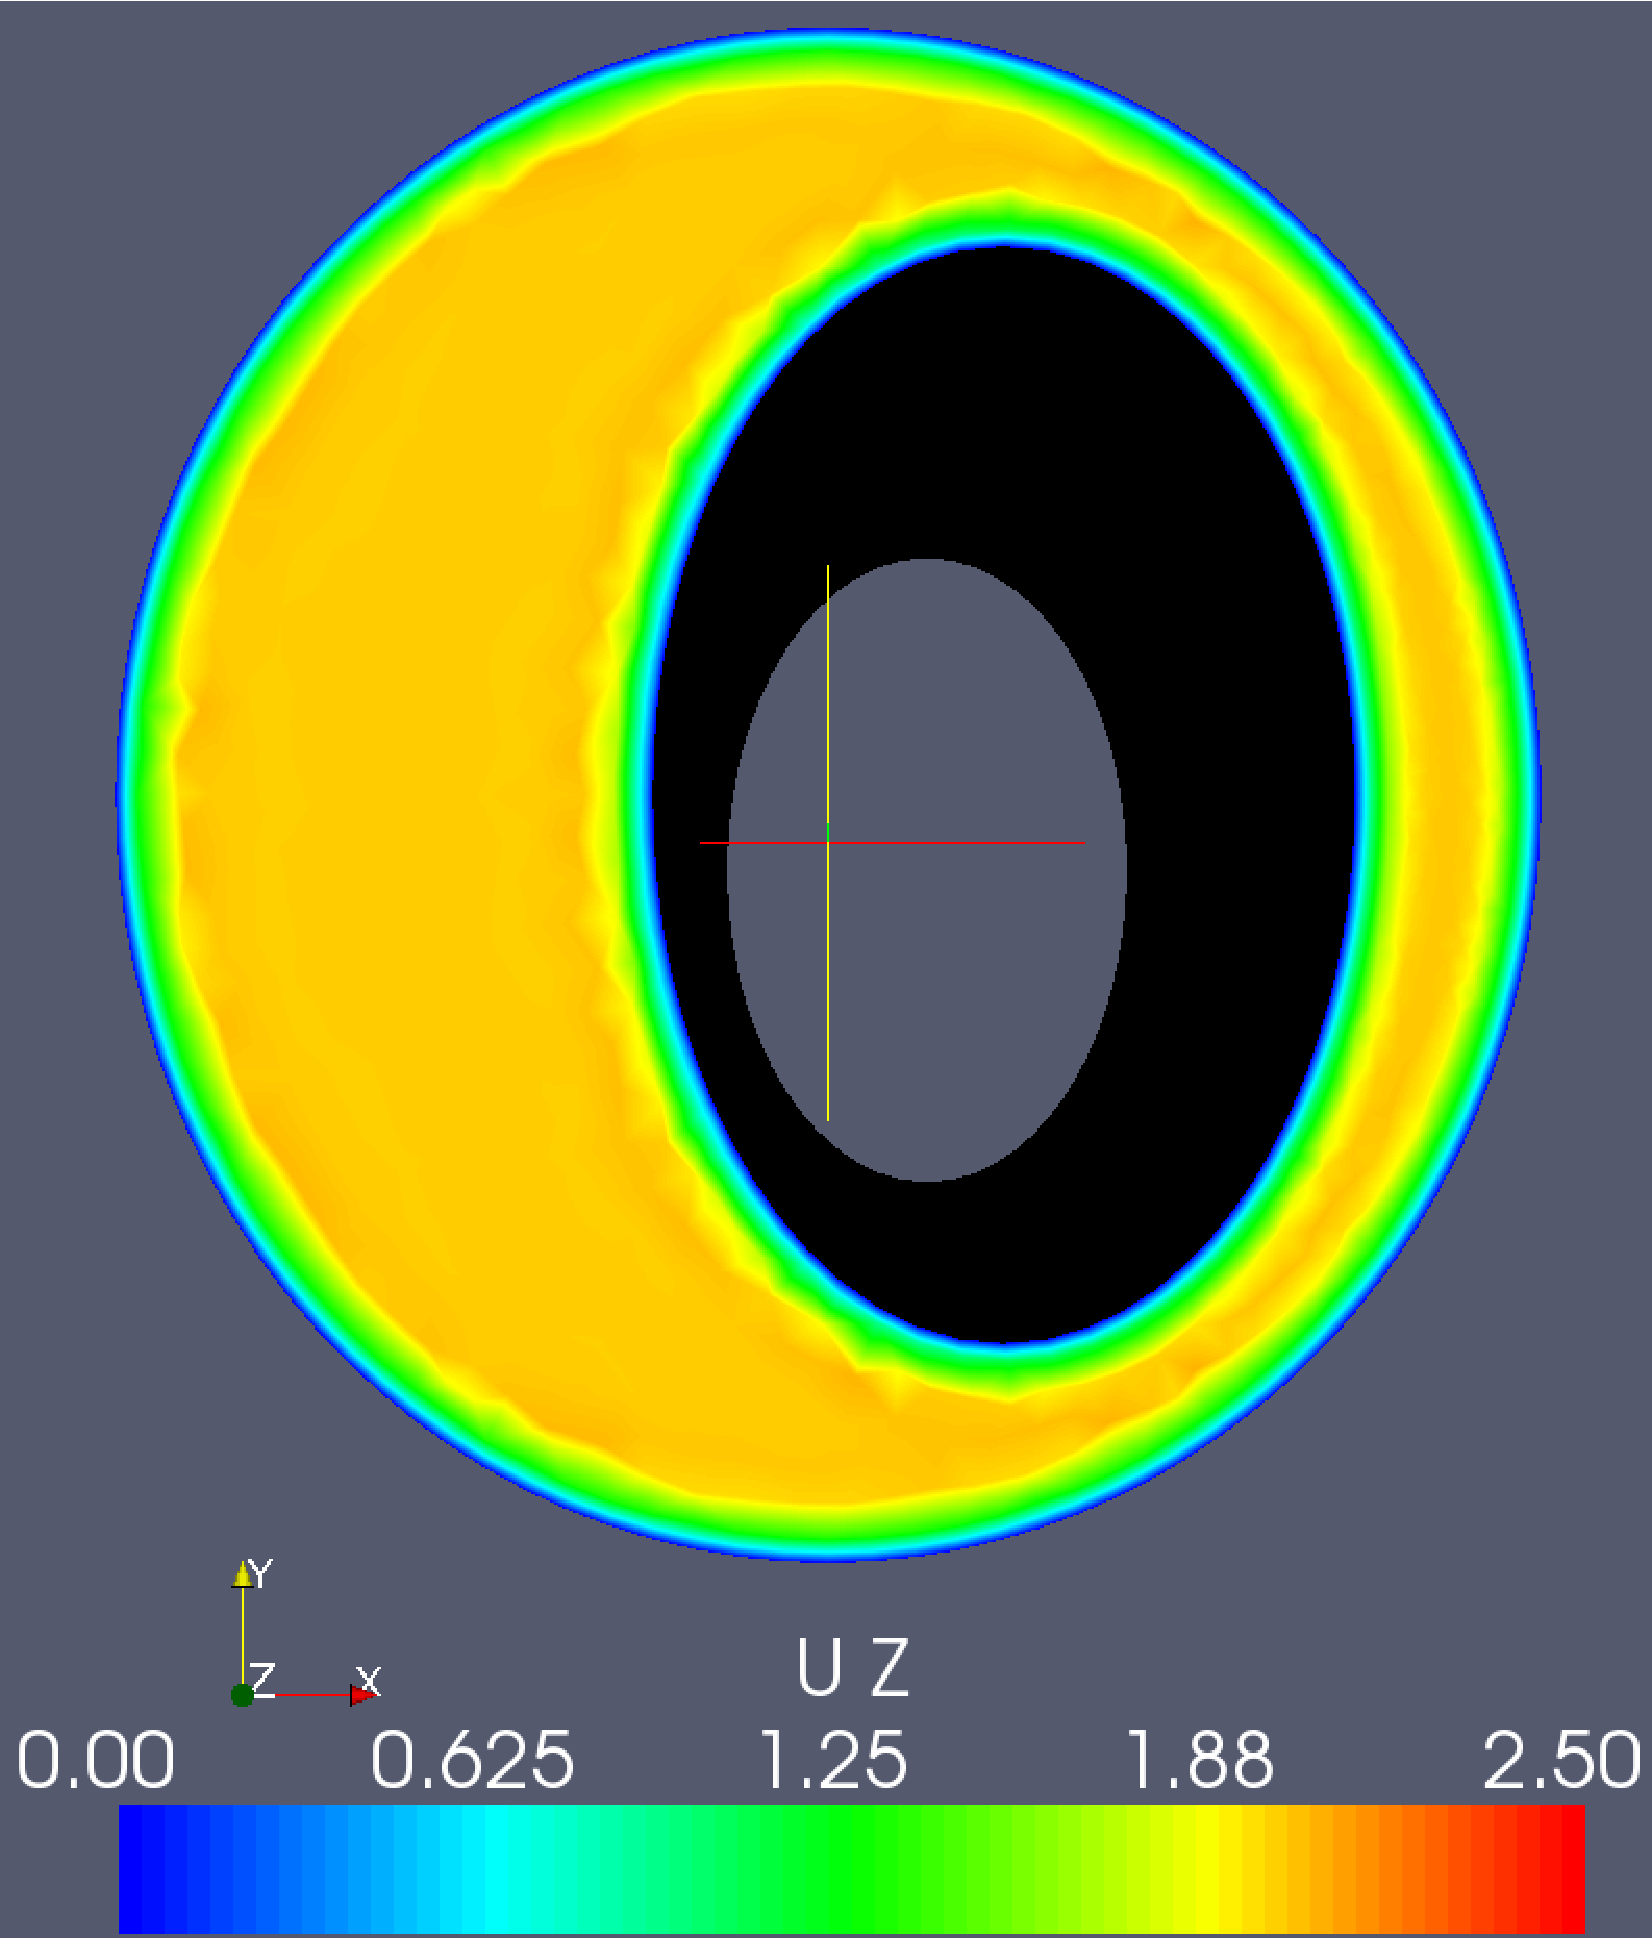
\includegraphics[width=\threefigsfull]{chapters/hentschel/pdf/pulse_f1_08_elliptic_eccentric_sysmax_nmb7.pdf}
            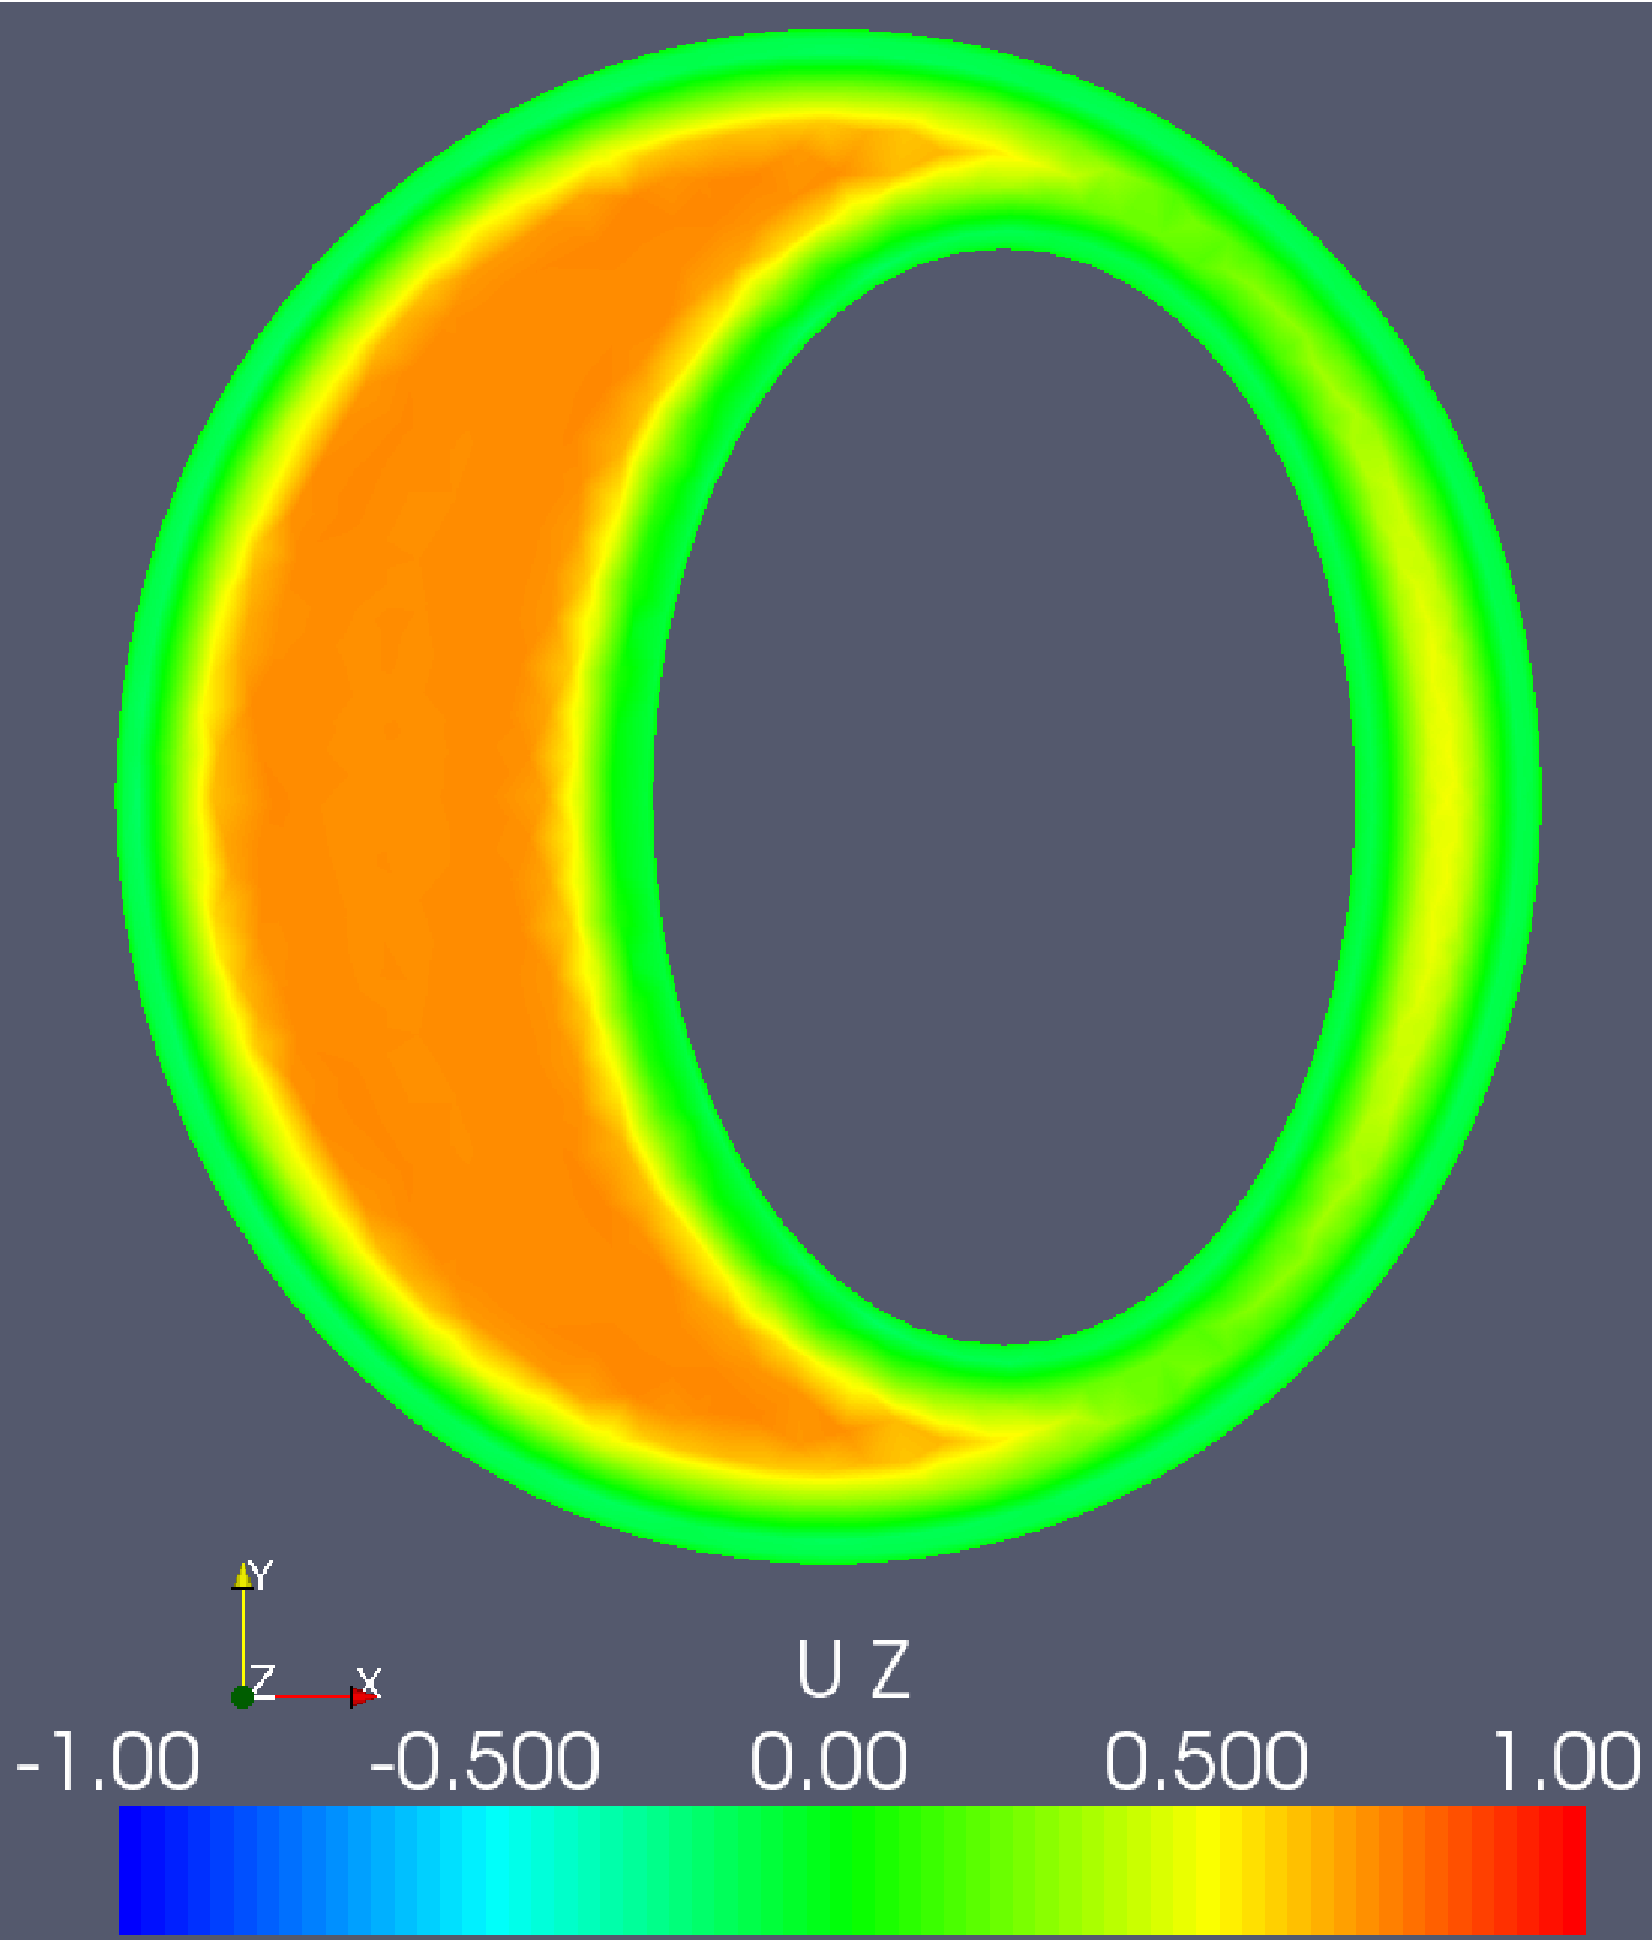
\includegraphics[width=\threefigsfull]{chapters/hentschel/pdf/pulse_f1_08_elliptic_eccentric_sysdia_nmb18.pdf}
            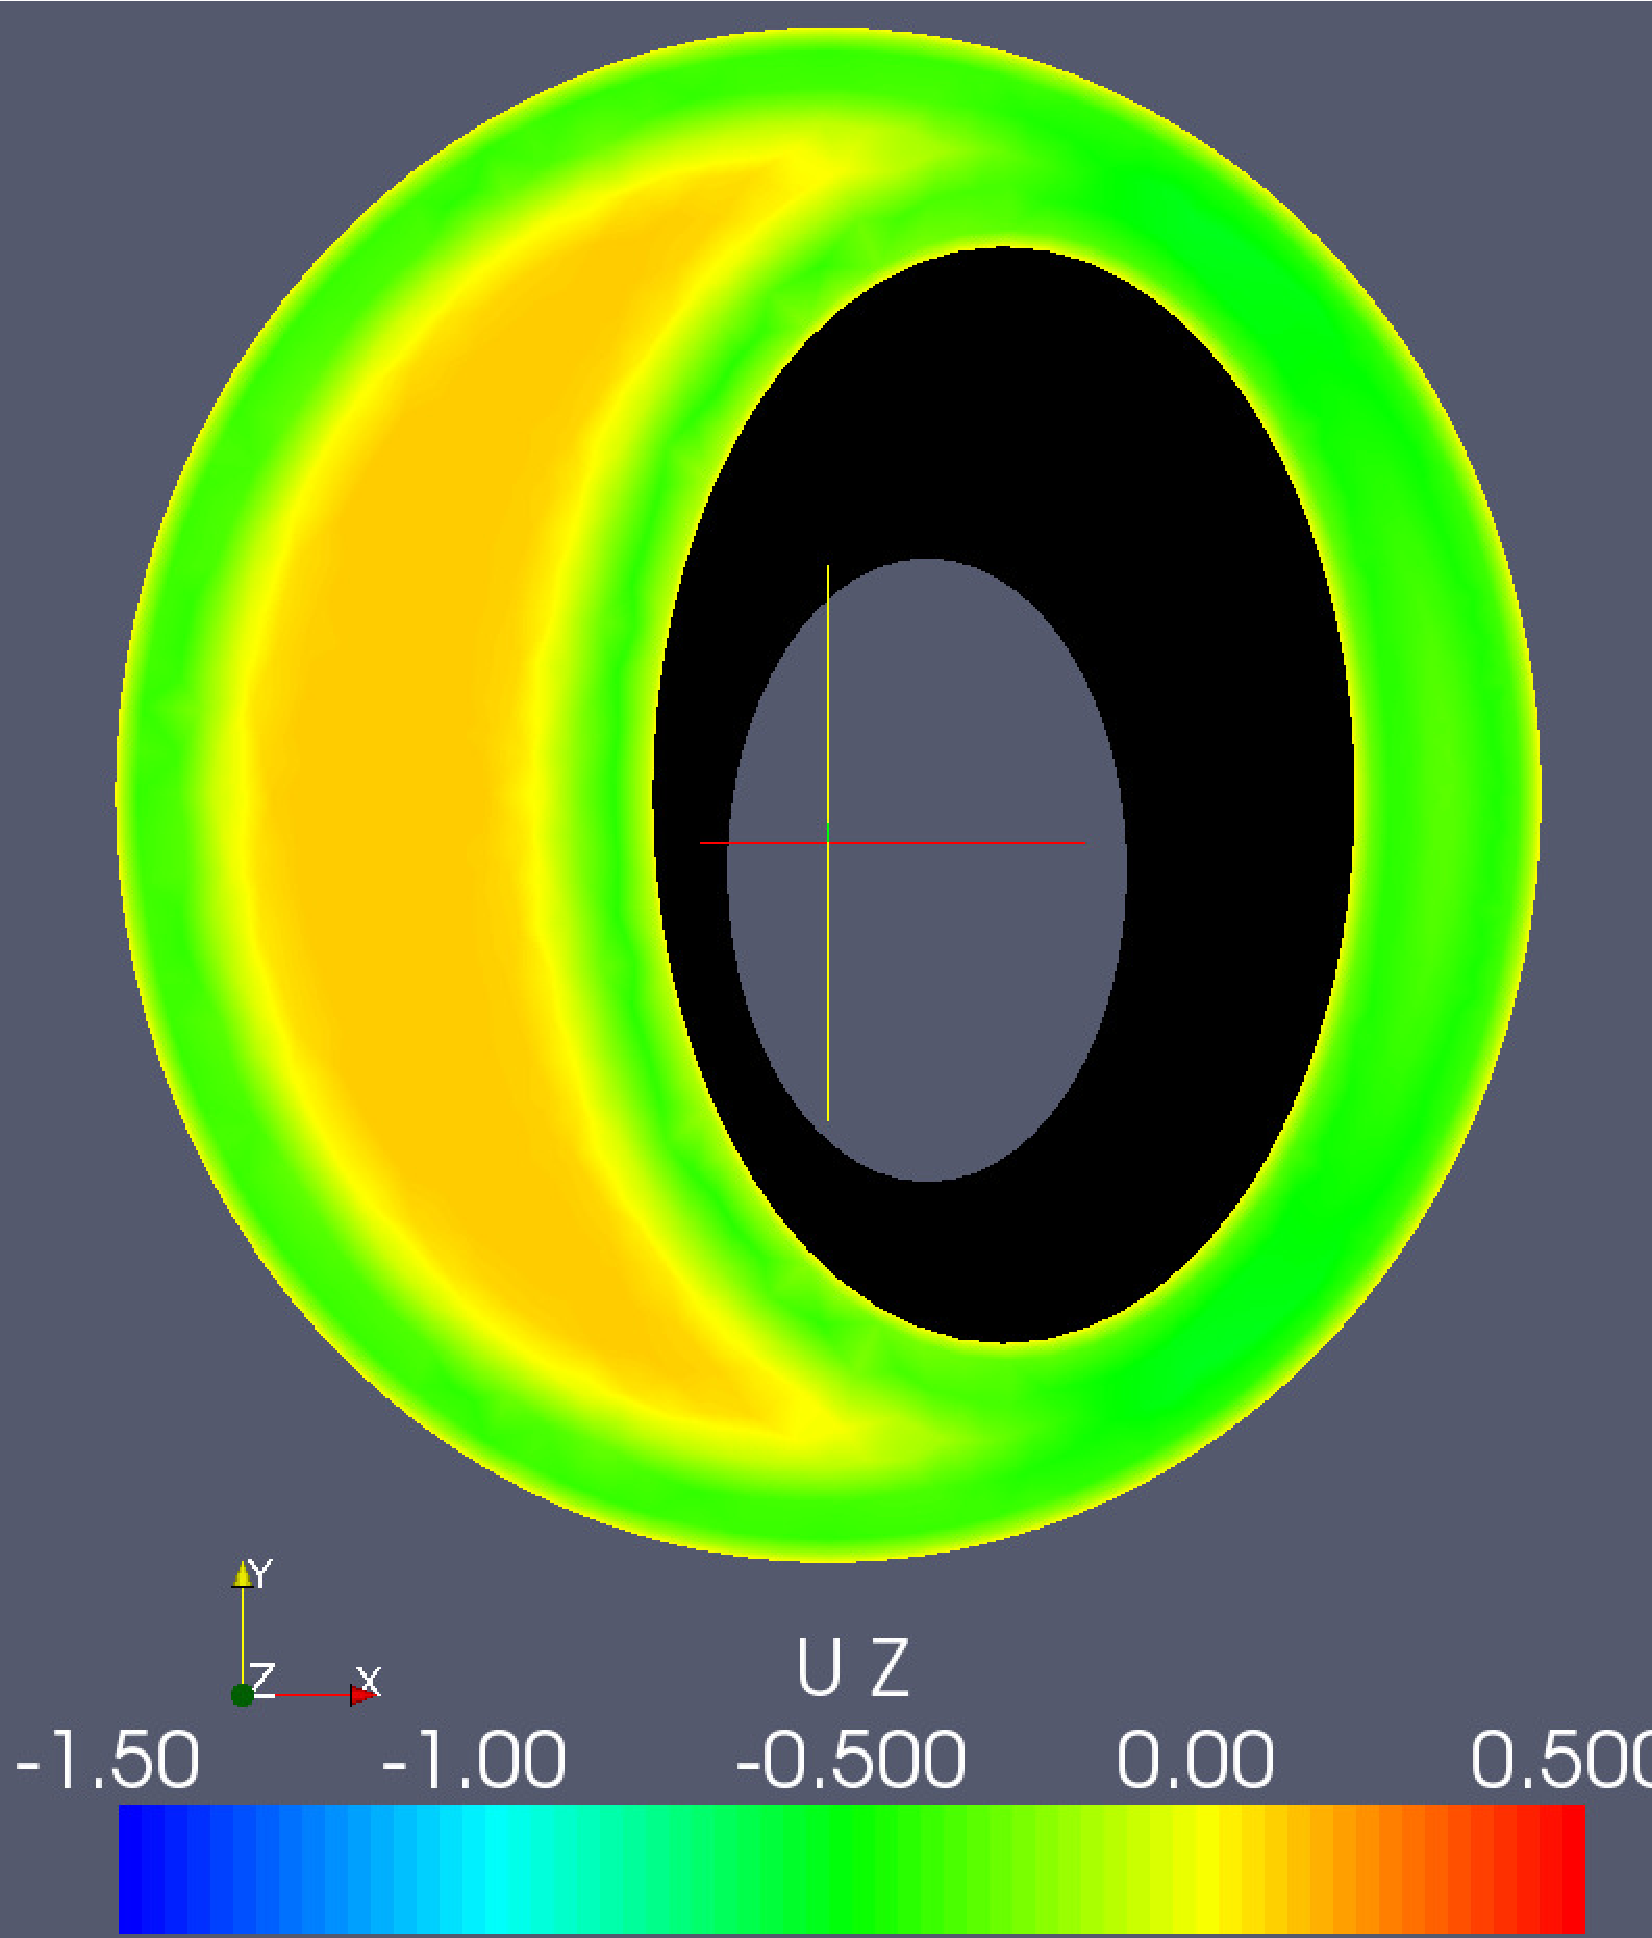
\includegraphics[width=\threefigsfull]{chapters/hentschel/pdf/pulse_f1_08_elliptic_eccentric_diamin1_nmb25.pdf}}
\end{figure}

\subsection{Example 4: cord with syrinx}

Syrinxes expand the cord so that it occupies more space of the spinal
SAS. Increasing the cord radius from 4 mm to 5 mm~\footnote{Similar to
setting the variables c and d in the geo-file to 0.5.} decreases the
cross sectional area by almost one third to 0.64 $\mathrm{cm^2}$. The
resulting flow is shown in Figure~\ref{fig:case4}. Apart from the
increased velocities, we see bidirectional flow already at t = 0.18 s
and at t = 0.25 s as before. The fact that diastolic back-flow is
visible at t = 0.18 s, shows that the pulse with its increased
amplitude travels faster.

\begin{figure}
\bwfig
  \ffigbox{\caption{The case with an enlarged cord diameter and the
      boundary conditions based on the pressure pulse. The pictures
      show the velocity in z-direction for the non-symmetric pulse at
      the time steps $t=0.07s, 0.18s, 0.25s$.}\label{fig:case4}}
          {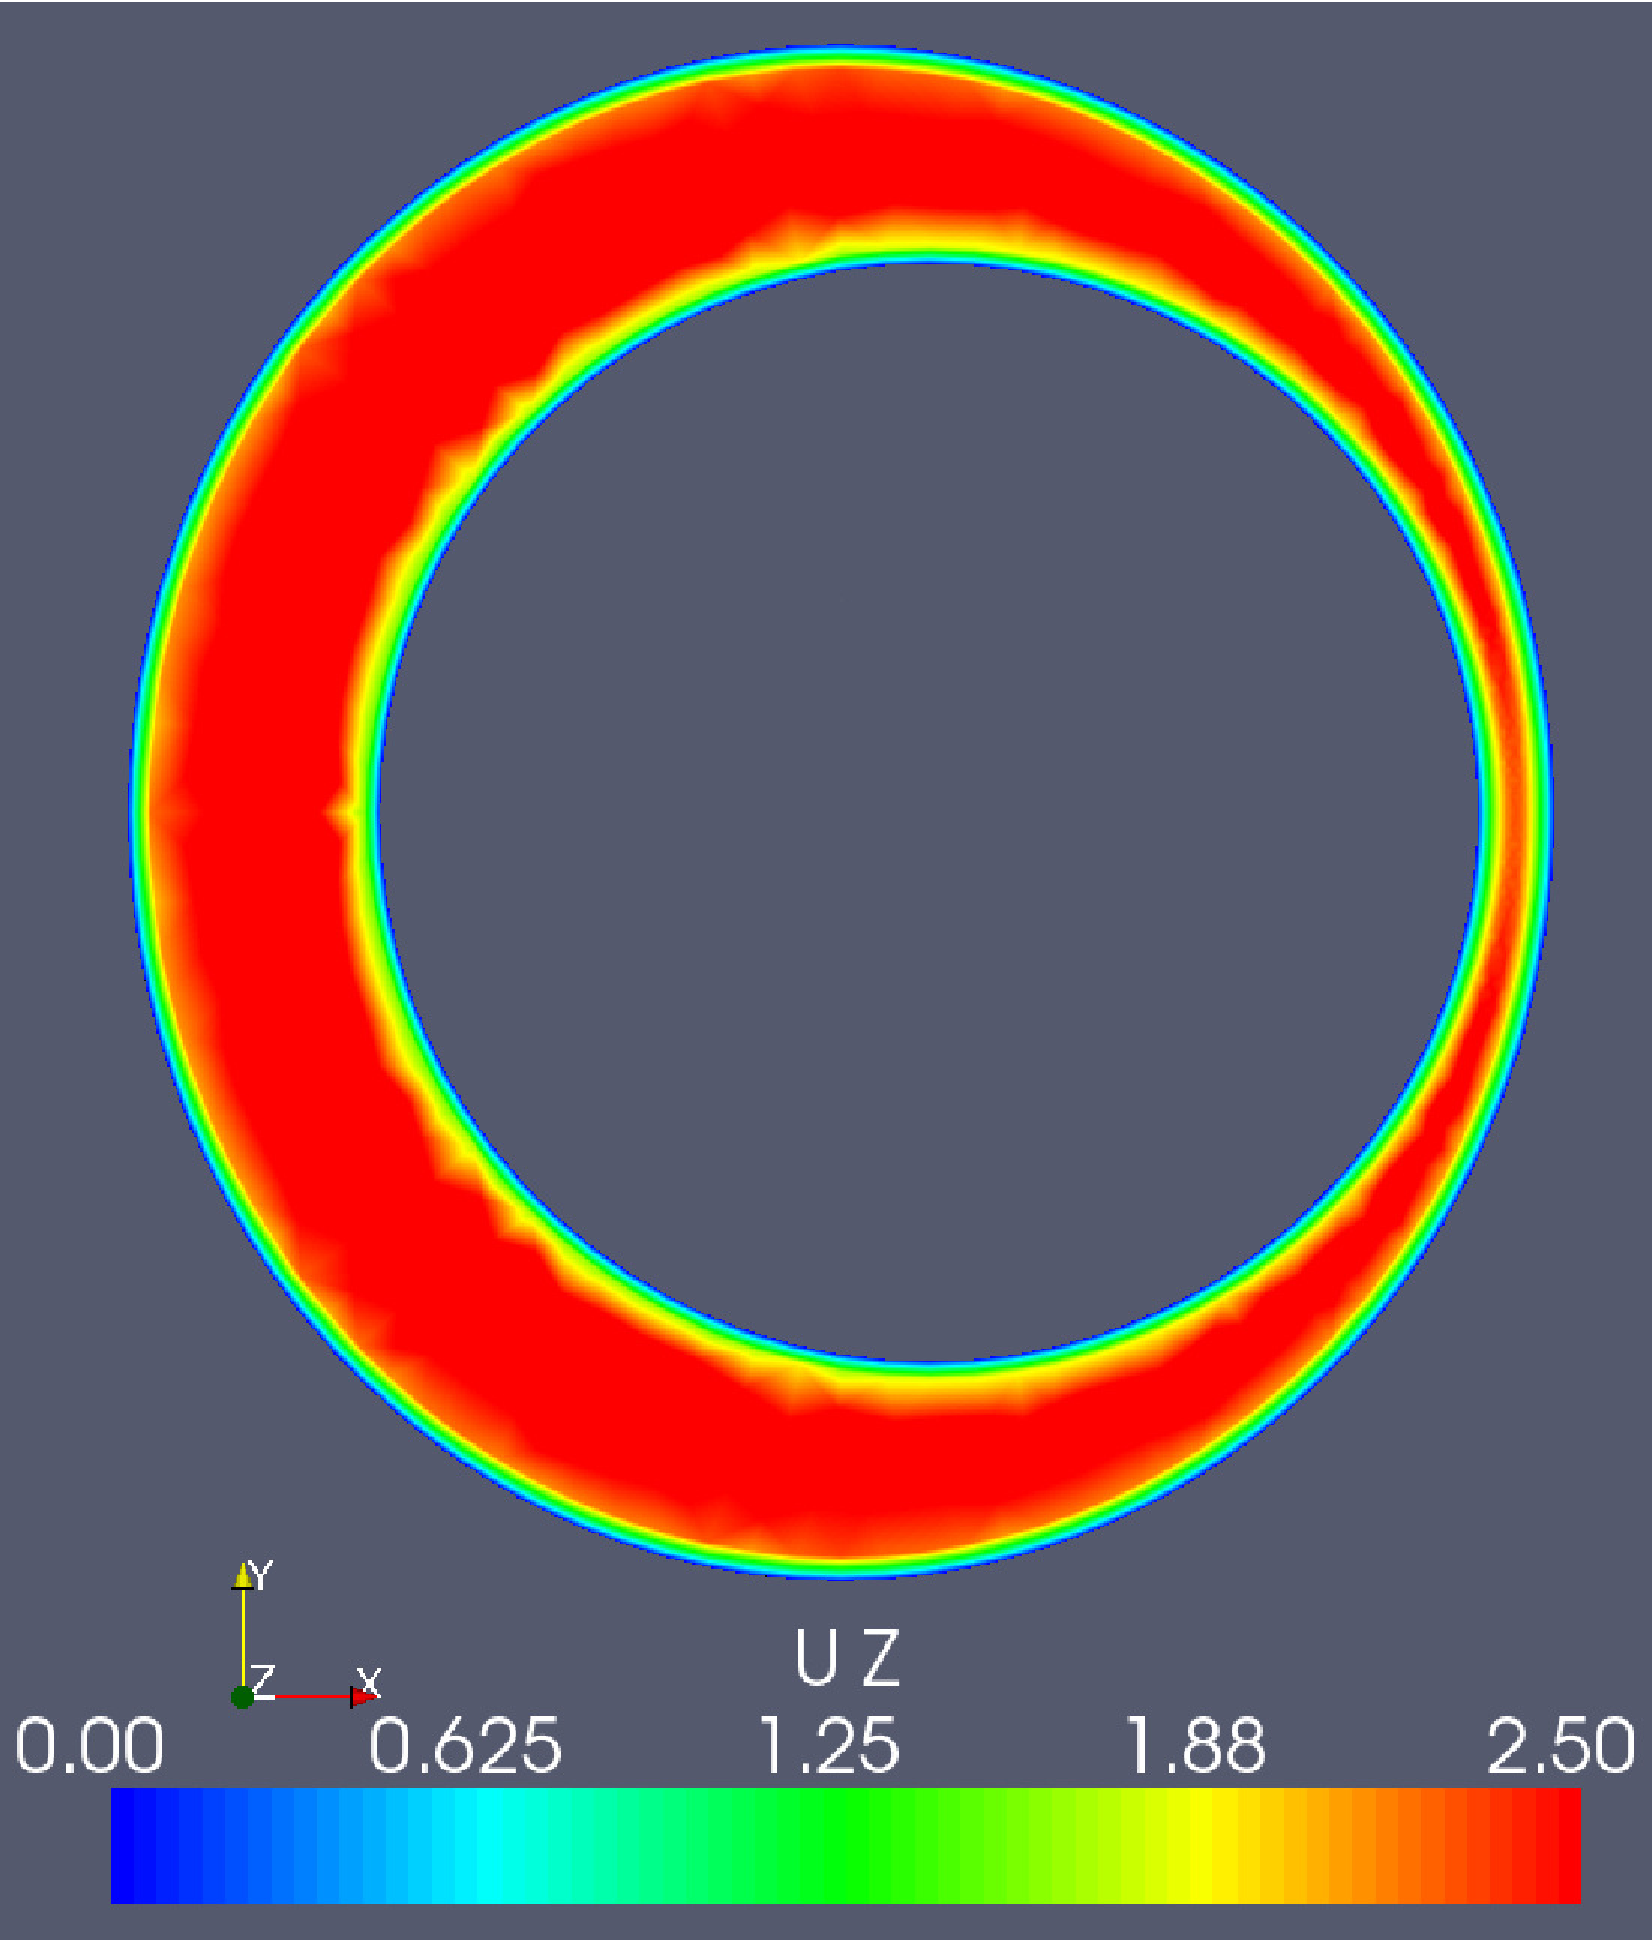
\includegraphics[width=\threefigsfull]{chapters/hentschel/pdf/pulse_syrinx_f1_08_syrinx05_sysmax_nmb7.pdf}
            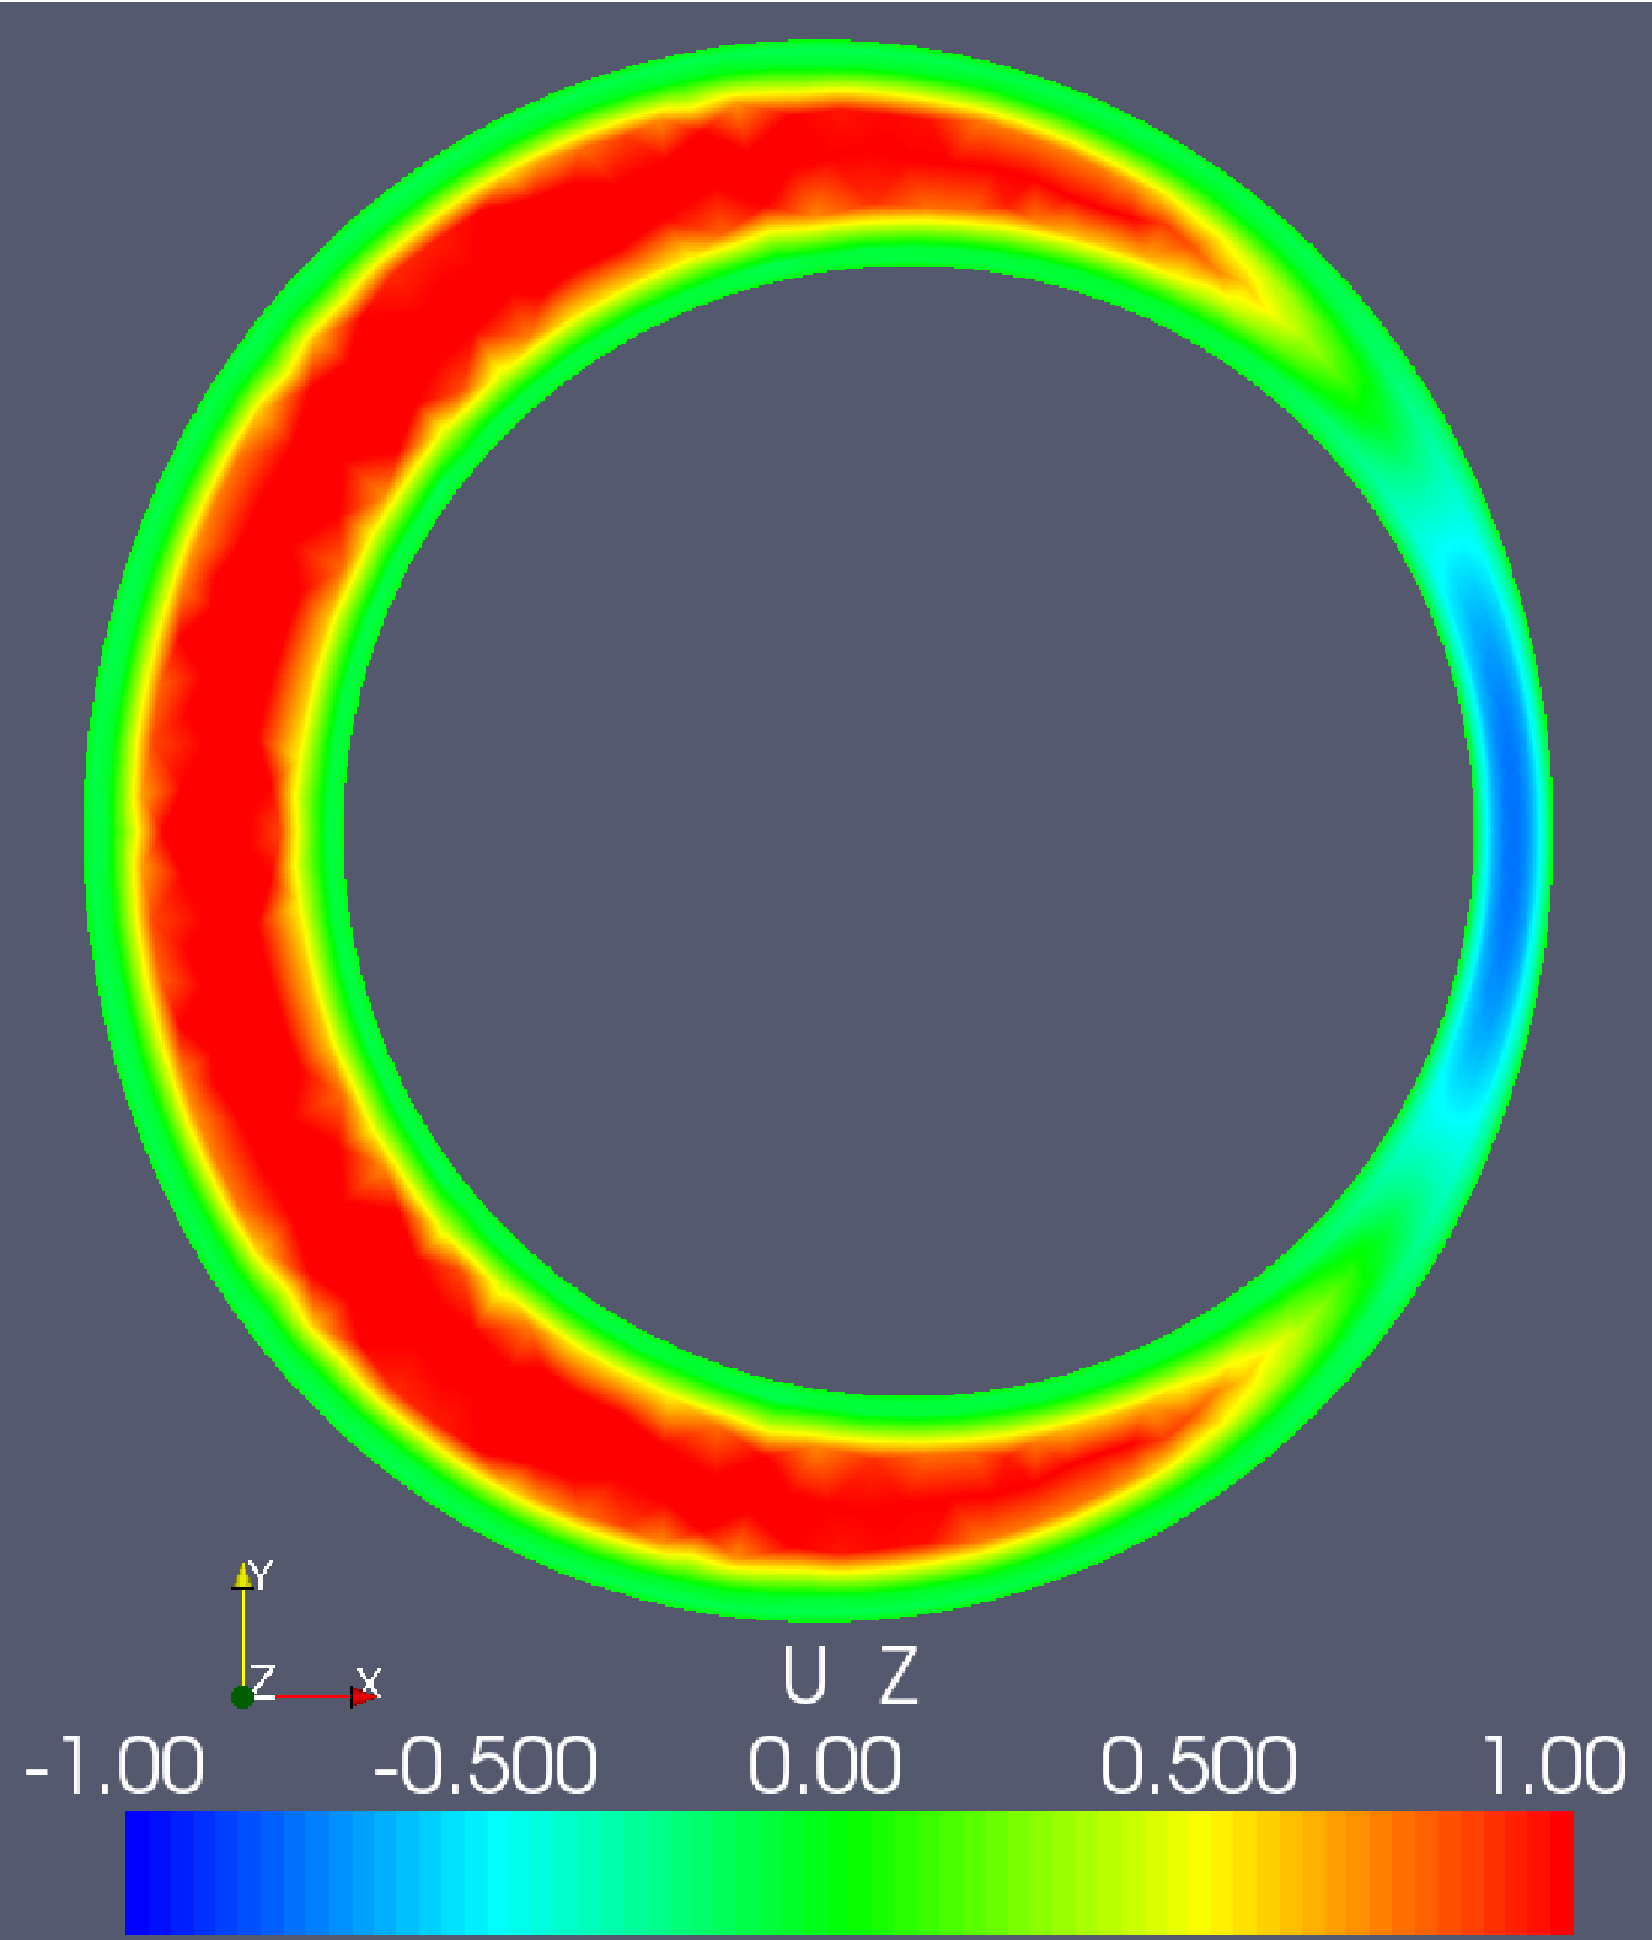
\includegraphics[width=\threefigsfull]{chapters/hentschel/pdf/pulse_syrinx_f1_08_syrinx05_sysdia_nmb18.pdf}
            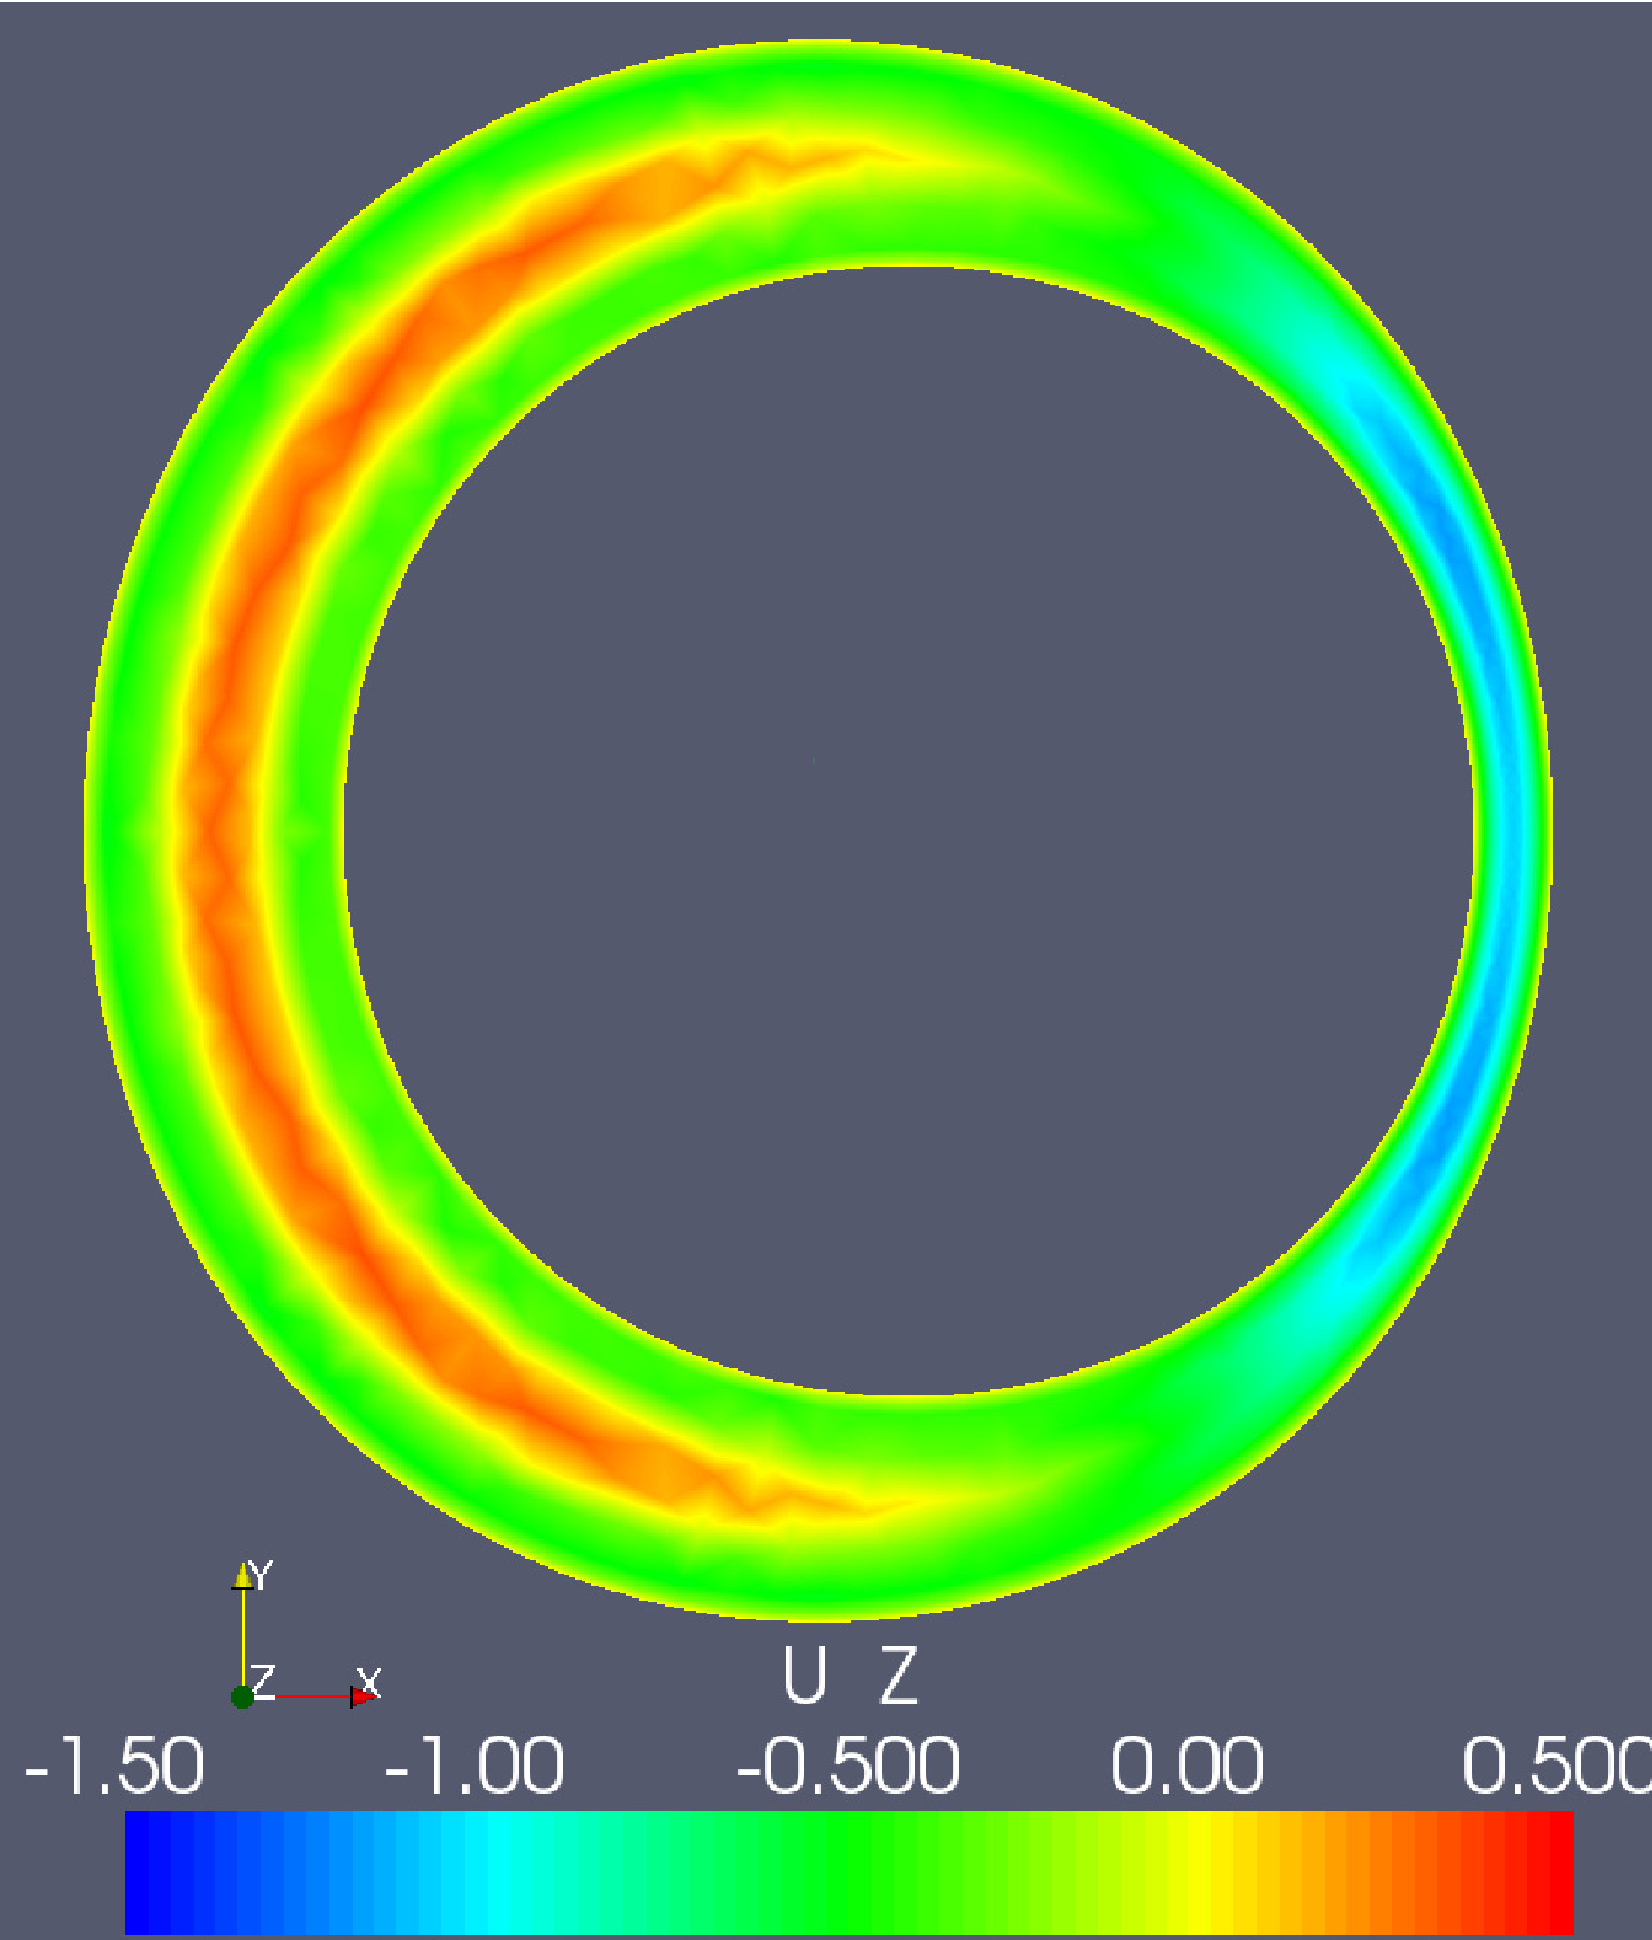
\includegraphics[width=\threefigsfull]{chapters/hentschel/pdf/pulse_syrinx_f1_08_syrinx05_diamin1_nmb25.pdf}}
\end{figure}

Comparing Reynolds and Womersley numbers shows a clear difference for
the above described examples 1, 2 and 3. Example 2 is marked by a
clearly lower maximum velocity at inflow and outflow boundary that
leads to a rather low Reynolds number. Due to the different inflow and
outflow area, example 4 has a lower Womersley number, leading to an
elevated maximum velocity at the boundary and clearly increased
Reynolds number. These numbers help to quantify the changes introduced
by variations in the model. For the chosen model, the shape of the
pulse function at the boundary as well as the cross sectional area
have great influence on the simulation results.
Comparison of Reynolds numbers
for different scenarios can be found in Table~\ref{tab:Re_We}.

\begin{table}
  \centering
  \begin{tabular}{ccccc}
    \toprule
    Problem & $D$ ,  in cm & $\mathbf{v}_{max}$ in cm/s  & $Re$ & $We$ \\
    \midrule
    Example 1 	&	0.54 & 2.3 & 177 & 17	\\
    Example 2	&	0.54 & 0.92 & 70 & 17	\\
    Example 4	&	0.45 & 3.2 	& 205 & 14	\\
    \bottomrule
  \end{tabular}
  \caption{Characteristic values for the examples 1, 2 and 3. Here,
    the characteristic length is $D=\sqrt(A/\pi)$, where $A$ is the
    inflow and outflow area.  Furthermore, $\mathbf{v}_{max}$ is
    defined as the maximal velocity at inflow and outflow boundary.}
  \label{tab:Re_We}
\end{table}

\section{Conclusion}

In this chapter, we have presented the use of FEniCS to simulate CSF
flow in various idealized geometries representing the spinal cord and
the surrounding subarachnoid space. We have further quantified the
effect of abnormal geometries and boundary conditions in terms of
pressure and flow deviations. From our simulations, it seems that
pressure instabilities are quickly damped out under realistic Reynolds
and Womersley numbers. These instabilities travel less than 1 cm and
it seems unlikely that Chiari induced pressure instabilities will
produce cysts several centimeters further down in the spinal canal.
We have observed that the velocity changes quite a bit with varying
shape and position of the cord. The pressure does, however, not change
much. The size of the cross section area does have an impact on the
pressure, as expected.  Finally, we observed that the pressure
computed using the G2 method differed significantly from the pressure
computed by Chorin and IPCS.
